\documentclass[11pt,a4paper]{article}
\usepackage[margin=24mm,headheight=14pt]{geometry}
\usepackage[T1]{fontenc}
\usepackage[utf8]{inputenc}
\usepackage{lmodern,microtype}
\usepackage{amsmath,amssymb,amsthm,mathtools}
\usepackage{booktabs,longtable,array,enumitem}
\usepackage{graphicx,xcolor,listings,fancyhdr}
\usepackage[hyphens]{url}
\usepackage[numbers,sort&compress]{natbib}
\usepackage[colorlinks=true,linkcolor=navy,citecolor=teal,urlcolor=navy,
  pdftitle={Toward Quasi-Polynomial Unknot Recognition},
  pdfauthor={Research continuation for the ProveIt project}]{hyperref}
\definecolor{navy}{HTML}{173B59}
\definecolor{teal}{HTML}{087E8B}
\definecolor{lightgray}{HTML}{F3F5F6}
\definecolor{muted}{HTML}{52616D}
\newtheorem{theorem}{Theorem}[section]
\newtheorem{lemma}[theorem]{Lemma}
\newtheorem{proposition}[theorem]{Proposition}
\newtheorem{corollary}[theorem]{Corollary}
\theoremstyle{definition}
\newtheorem{definition}[theorem]{Definition}
\theoremstyle{remark}
\newtheorem{remark}[theorem]{Remark}
\newcommand{\F}{\mathbb{F}_2}
\newcommand{\poly}{\operatorname{poly}}
\newcommand{\code}[1]{\texttt{#1}}
\newcolumntype{P}[1]{>{\raggedright\arraybackslash}p{#1}}
\lstset{basicstyle=\small\ttfamily,backgroundcolor=\color{lightgray},
  frame=single,rulecolor=\color{lightgray},breaklines=true,
  columns=fullflexible,keepspaces=true,showstringspaces=false,
  xleftmargin=4pt,xrightmargin=4pt,aboveskip=10pt,belowskip=10pt}
\setlist{topsep=4pt,itemsep=3pt,parsep=0pt}
\setlength{\emergencystretch}{2em}
\pagestyle{fancy}
\fancyhf{}
\fancyhead[L]{\small\color{muted}ProveIt / Unknot recognition}
\fancyhead[R]{\small\color{muted}Research continuation, October 2026}
\fancyfoot[C]{\small\thepage}
\renewcommand{\headrulewidth}{0.3pt}
\title{\color{navy}\bfseries Toward Quasi-Polynomial\\Unknot Recognition\\[6pt]
  \large Certified Factorization, Sparse Elimination,\\
  Pointed Khovanov Scanning, and Explicit Complexity Obligations}
\author{Research continuation for Vladimir Reshetnikov's ProveIt project}
\date{7 October 2026\\[3pt]\small Source baseline:
  \texttt{4e6fe879e5238ec0b134b6d33fdca0b8c7c1c711}}

\begin{document}
\maketitle
\begin{abstract}
We continue the performance work on ProveIt's exact unknot recognizer with
three implemented improvements and a revised complexity analysis.  A certified
interlacement decomposition replaces recursively reconstructed visible
connected sums.  Its combinatorial core uses $O(n\alpha(n))$ time and linear
space; the checked PD interface uses $O(n\log(n+1))$ time.  We prove that a
specific family forces quadratic crossing work in the archived factorizer.
An incidence-indexed finite-field determinant replaces dense elimination on
large Alexander minors and admits an explicit bound in terms of measured
Schur-complement work.  An optional pointed scanner computes reduced Khovanov
homology directly, with a basepoint policy preserving every proper-prefix
frontier size and an exact decision-only early-stop rule.

We also correct a consequential complexity assertion: arbitrary scan frontiers
need not have Catalan-many matching states.  A six-crossing validated diagram
and a default-order repository fixture provide exact counterexamples.  We
state the safe general bound, the additional disk hypothesis that restores
Catalan counting, and a parameterized recognition bound that exposes the
independent multiplicity obstruction.  For a possible hierarchy backend we
prove a sharp mixed-radix suffix-reconstruction budget and an explicit
conditional quasi-polynomial theorem.

The deliverable includes runnable code, independent verification programs,
raw randomized paired timings, an exact archived baseline, and an integration
patch.  Large constructed inputs show substantial speedups; the pointed
scanner has mixed timing results and remains opt-in.  No general
quasi-polynomial unknot-recognition bound is established.  The final research
agenda identifies the geometric, algebraic, and bit-complexity results that
would be needed to establish one.
\end{abstract}
\vspace{5pt}
\noindent\textbf{Keywords.} Unknot recognition; visible connected sums;
interlacement; sparse elimination; reduced Khovanov homology; frontier width;
normal surfaces; hierarchy complexity; reproducible computation.
\clearpage
\tableofcontents
\clearpage

\section{Results, scope, and the research objective}
\label{sec:introduction}

The objective is a sound and complete recognition algorithm whose worst-case
running time on an $n$-crossing knot diagram is quasi-polynomial.  We use
\emph{quasi-polynomial} in its usual broad sense
$\exp((\log n)^{O(1)})$, and distinguish the sharper target
\begin{equation}
 T(n)=n^{O(\log n)}=\exp(O(\log^2 n)).
 \label{eq:main-target}
\end{equation}
Logarithms may be taken in any fixed base greater than one.  To avoid small
input exceptions, an asymptotic expression involving $\log n$ can always be
read with $\log(n+2)$.

The present continuation makes concrete progress in the repository's
implemented pipeline and sharpens the statements needed to connect that work
to \eqref{eq:main-target}.  It does not identify fast behavior on a sample
with a worst-case theorem.  Nor does it use a one-sided knot invariant as an
unknot certificate.  Each claim below is assigned to its actual logical role.

\subsection{What is established here}

\begin{enumerate}[leftmargin=*,label=\arabic*.]
\item \textbf{A provable preprocessing improvement.}  The new factorizer
computes the atomic visible summands through connected components of the
Gauss-word interlacement graph without constructing its potentially quadratic
edge set.  A short spanning forest and a separate nesting check certify the
partition.  The checked implementation is nearly linear, and a specified
embedding of cyclic trefoil sums forces quadratic work in the old recursive
implementation.  The graph-theoretic correspondence is classical; its
integration, certificate format, reconstruction audit, and baseline comparison
are the contribution (Section~\ref{sec:factorization}).

\item \textbf{An exact sparse filter implementation.}  Alexander minors
already have sparse input rows.  We retain this structure through elimination
using both row dictionaries and column incidence sets.  The work depends on
the actual pivot neighborhoods.  Worst-case cubic arithmetic remains possible;
the new bound explains when sparse inputs give a benefit and why input sparsity
alone is insufficient (Section~\ref{sec:sparse}).

\item \textbf{A direct reduced backend with decision semantics.}  The pointed
quotient removes one dot variable from each relevant Hom space.  A last-crossing
basepoint policy avoids the extra frontier size introduced by an early cut.
Two isolated partial-complex summands prove knottedness before full homology
is necessarily known.  The engine is implemented and independently checked,
but remains optional because some small cases become slower
(Section~\ref{sec:pointed}).

\item \textbf{A corrected interface bound.}  The old Catalan assertion for
arbitrary matching dictionaries is false, including on an existing fixture
under the actual default ordering.  We supply exact coefficients, independent
reconstruction, and the appropriate replacement theorem.  This is a correction
to the resource analysis, not evidence that the bracket values on those
examples are wrong (Section~\ref{sec:frontiers}).

\item \textbf{Quantitative conditions for the target.}  The scan analysis
separates boundary width from object multiplicity.  The hierarchy analysis
separates termination, encoded state volume, constructive cost, and repeated
reconstruction.  A sharp suffix-work formula improves the accounting but
does not supply the missing geometric algorithms
(Sections~\ref{sec:parameters} and~\ref{sec:hierarchy}).
\end{enumerate}

\subsection{The exact source baseline}

The baseline is the \path{Topology/UnknotRecognition/fast} subtree of
ProveIt at revision
\begin{center}\small
\texttt{4e6fe879e5238ec0b134b6d33fdca0b8c7c1c711}.
\end{center}
It was inspected on 7 October 2026, together with the repository's synthesis
and acceleration-proposal material~\cite{repository}.  The archived package
already includes much of the earlier optimization work: incremental
Reidemeister I/II reduction, a descending-diagram test, visible connected-sum
factorization, modular Alexander and Jones obstructions, optional exact
Alexander computation, delayed Reidemeister III search, and a highly optimized
Bar--Natan scanner.  Its scan has interned matching geometry, bit-packed
morphisms, compiled gluing plans, min-fill pivot heuristics, cache reuse,
optional delayed final cancellation, and optional races between orders.

Consequently, comparison with a generic cube-of-resolutions implementation
would overstate the engineering advance.  Our timing baseline is the actual
archived package.  Its 40 selected source, example, and test files are retained
byte-for-byte, checked against their Git blob hashes.  Historical timing output
is not required to execute that package.  Independent-module loading prevents
an accidental comparison of the updated code with itself.

The proposed Python package version is 0.3.0.  The archive contains both a
complete updated package and a patch against the pinned source.  The existing
Rust port has not been changed.  We do not present a Python improvement as an
already implemented cross-language improvement.

\subsection{Why the current recognition decision remains exact}

A nonunit Alexander minor or a Jones evaluation differing from the unknot
value certifies knottedness.  Passing those filters is inconclusive.  A
descending diagram certifies the unknot, and a visible connected sum is trivial
exactly when all its summands are trivial.  The residual exact test uses
reduced Khovanov rank one.  Khovanov unknot detection supplies the needed
topological characterization~\cite{kronheimermrowka}.  The implication from
rank one over $\F$ to rank one over $\mathbb Q$ follows from universal
coefficients and nonvanishing; the unknot has reduced rank one over either
field.  Thus the characteristic-two implementation has the same decision
criterion.

With no imposed resource limits the finite scanning computation is complete.
Cooperative time or object ceilings can yield \code{UNKNOWN}; they never
justify \code{UNKNOT} or \code{KNOTTED}.  The new early decision API reports a
proved lower bound separately from an exact rank.  These distinctions are
maintained at the code and evidence interfaces.

\section{Input, cost model, and notation}
\label{sec:model}

A PD code specifies four cyclically ordered ports at each crossing, with the
same over/under convention as the repository.  Validation checks two
occurrences per edge label, a single traversed strand, and a spherical rotation
system.  For a connected $n$-crossing projection with $n>0$, there are $n$
vertices and $2n$ edges; the spherical face condition is $n+2$ faces.  The
zero-crossing input denotes the trivial circle by convention.  Braid and grid
inputs first expand to PD codes, so all crossing-count bounds refer to the
expanded diagram.  A bound in a more succinct original encoding must include
the conversion cost and output size.

We normalize edge labels to indices of $O(\log(n+2))$ bits.  Combinatorial
RAM bounds assume word-sized indices, as is standard for graph algorithms.
If arbitrary long external labels are supplied, reading and normalization
also depend on their total encoded length.  The hierarchy theorem instead
states bit-cost obligations explicitly because normal coordinates can be
exponentially large integers even when the input triangulation is small.

Let $w_i$ be the number of frontier endpoints after $i$ scanned crossings,
and $w=\max_i w_i$.  Let $M$ be the largest number of live objects after a
fully cancelled stage of a specified scan, including its initial and final
stages.  The maximum multiplicity of one boundary matching, summed over
homological degrees, will be denoted by $\mu$.  Neither $M$ nor $\mu$ is
bounded by counting different matchings.  The scalar Jones filter has only
one field coefficient per matching, whereas the homological scanner can have
many objects with that same matching.

For finite-field elimination, $m$ is matrix dimension, $E$ is the number of
stored input entries, $Z_{\max}$ is the largest active nonzero count, and $F$
is the cumulative number of Schur-update positions.  These matrix symbols
are distinct from the crossing count $n$.  The modular filters use the fixed
prime $p=2^{61}-1$.  Their arithmetic is exact in $\mathbb F_p$; fixed
evaluation points provide no distributional success guarantee against an
adversarial family.

When stating an implementation bound using dictionaries and sets we use the
standard bounded-cost lookup model.  Python's hashing behavior is not being
promoted to a deterministic worst-case data-structure theorem.  Ordered
maps can supply deterministic alternatives at additional logarithmic cost.
Wall-clock measurements are reported separately from operation counts.

\section{Certified visible factorization through interlacement}
\label{sec:factorization}

Visible connected sums provide a useful opportunity to replace repeated
geometric reconstruction by a single combinatorial computation.  The
underlying correspondence is established mathematics: connected-sum
decomposability of a planar curve is characterized by disconnectedness of
its interlacement graph \cite{khan2021}.  Courcelle's atomic decomposition
places the related word and graph decompositions in a broader framework
\cite[Definition~22 and Lemma~23]{courcelle}.  Computing overlap components
without constructing all overlap edges also has precedents, including
linear-time methods discussed by Schmidt \cite[Section~4.1 and Lemma~15]{schmidt}.
Our contribution here is a concrete certified implementation, its precise
relationship to the existing PD factorizer, and an exact family exhibiting
quadratic work in that implementation.  We give the necessary proofs because
the spherical embedding, crossing data, certificate format, and reconstruction
cost all matter for a correct replacement.

\subsection{Words, gaps, and geometric cuts}

Fix a validated spherical one-component PD diagram $D$ with $n>0$ crossings.
Following its strand through opposite crossing ports gives a cyclic word
$W$ of length $2n$, with each crossing label occurring twice.  After fixing
a starting position, write $p_x<q_x$ for the positions of label $x$.

\begin{definition}
The interlacement graph $I(W)$ has the crossing labels as vertices, and
distinct labels $x,y$ are adjacent precisely when
\begin{equation}
\label{eq:interlacement}
p_x<p_y<q_x<q_y
\quad\text{or}\quad
p_y<p_x<q_y<q_x.
\end{equation}
A cyclic interval of visits is \emph{closed} if every label occurring in it
has both occurrences there.  A \emph{visible split} uses a Jordan curve in
the projection sphere meeting the diagram transversely in exactly two edge
interiors, with at least one crossing on each side.
\end{definition}

The adjacency relation is independent of the starting position and of
traversal reversal.  In a chord picture it says exactly that the endpoints
of the two chords alternate.

\begin{lemma}[Gap property]
\label{lem:interlace-gaps}
If $C$ and $E$ are distinct connected components of $I(W)$, all endpoints
of $E$ belong to a single gap between consecutive endpoints of $C$ on the
circle.  Consequently, their first-to-last endpoint intervals in a linear
reading are disjoint or nested.  A nested interval contains no endpoint of
the outer component.
\end{lemma}

\begin{proof}
Take a chord $e\notin C$ with no neighbor in $C$.  Its endpoints divide the
circle into two open arcs.  Since no chord of $C$ alternates with $e$, both
endpoints of each chord of $C$ lie in one of these arcs.  Chords lying in
different arcs cannot alternate with one another.  Connectedness of $C$
therefore puts all its endpoints in the same arc.  The complementary arc
contains no endpoint of $C$, so the endpoints of $e$ belong to one gap of $C$.
Chords in different gaps of $C$ cannot interlace.  Connectedness of $E$ now
puts all its chords in a single gap.

For the linear assertion, suppose the first endpoint of $C$ precedes the
first endpoint of $E$.  If the latter follows the last endpoint of $C$,
the hulls are disjoint.  Otherwise it lies in a bounded internal gap of $C$;
the first assertion places all endpoints of $E$ in that gap.  This gives
the asserted nesting and exclusion of outer endpoints.
\end{proof}

\begin{lemma}[Closed intervals and two-edge cuts]
\label{lem:closed-visible-cut}
A nonempty proper closed interval of $W$ gives a visible split.  Conversely,
every visible split separates complete connected components of $I(W)$.
\end{lemma}

\begin{proof}
Let $A$ be the labels in such an interval.  Following the interval traverses
only crossings of $A$, and following its complement traverses only crossings
outside $A$.  Hence exactly the two boundary edges join $A$ to its
complement.  Both induced projection subgraphs are connected: each is
covered by the corresponding traversal segment.

Take a small regular neighborhood of the connected subgraph on $A$ in the
projection sphere.  Its boundary consists of disjoint circles crossing
only the two boundary edges.  The connected complementary subgraph lies
in one component of the neighborhood's complement, so both edges leave
through that component's boundary circle.  This circle supplies the
required visible split.  In the equivalent dual description, a two-edge
bond is a two-edge cycle.  Its two edges border the same two faces, which
are distinct because a connected Eulerian graph has no bridge.
Closing either traversal segment along the curve yields
a spherical one-component diagram; the crossing rotations and over/under
data on its side are preserved.

Conversely, traversal meets a visible splitting curve twice.  Between those
meetings it stays on one side, and the complementary traversal stays on the
other.  Both visits to each crossing lie on the same side.  The two sets of
labels therefore form closed intervals, so labels on opposite sides cannot
alternate.  No connected component of $I(W)$ can cross the partition.
\end{proof}

\begin{theorem}[Canonical visible factors]
\label{thm:interlace-factors}
Let $C_1,\ldots,C_k$ be the connected components of $I(W)$.  Every complete
recursive visible factorization has these atomic crossing sets.  The factor
$D[C_i]$ is specified by the induced cyclic traversal on $C_i$ and the
crossing rotations and under/over information inherited from $D$.  In
particular,
\begin{equation}
\label{eq:interlace-connected-sum}
K(D)=K(D[C_1])\mathbin{\#}\cdots\mathbin{\#}K(D[C_k]).
\end{equation}
The crossing sets and inherited factor diagrams are independent of the
chosen sequence of visible splits, up to edge labels and traversal choices.
\end{theorem}

\begin{proof}
If $k>1$, choose a component whose first-to-last interval contains no strictly
nested component interval.  Lemma~\ref{lem:interlace-gaps} shows that every
endpoint in this interval belongs to the chosen component.  It is a closed
proper interval, so Lemma~\ref{lem:closed-visible-cut} splits it off.  Deleting
these endpoints leaves all relative orders among the remaining endpoints
unchanged, hence leaves all remaining interlacement components unchanged.
Induction produces exactly the stated factors.

Conversely, Lemma~\ref{lem:closed-visible-cut} prevents any visible split
from dividing a connected interlacement component.  Once a factor has only
one component, no further visible split is possible.  Reconnection after
a split deletes the other traversal interval and introduces no crossing.
Thus any sequence ending with crossing set $C_i$ has the same induced
cyclic traversal and the same original crossing ports.  These determine its
PD incidences and rotation system.  The splitting curve gives a decomposing
sphere after thickening its disk in the ambient three-sphere, yielding
\eqref{eq:interlace-connected-sum} at every step.
\end{proof}

This is uniqueness for a fixed input diagram, including its rotations.
A Gauss word by itself need not determine all its planar realizations
\cite{courcelle}.  Nor does connectedness of $I(W)$ assert that the represented
knot is prime: a composite knot may have a diagram with no visible split.
Singleton interlacement components close to one-crossing curl factors.
The crossing-free circle, excluded from the preceding notation, is returned
as one factor.

\begin{remark}[Nested factors]
The realizable word
\[
a\,b\,c\,d\,b\,c\,d\,a\,e\,e
\]
has components $\{a\}$, $\{b,c,d\}$, and $\{e\}$.  The middle component is a
triangle of interlacement edges.  Its entire word lies in one gap of the
two endpoints of $a$.  One first removes that middle block and obtains
$a\,a\,e\,e$.  The atomic crossing sets are therefore not generally the
consecutive blocks of the original word.  The component computation handles
this nesting without recursively rebuilding diagrams.
\end{remark}

\subsection{Sparse discovery and its invariant}

Constructing $I(W)$ explicitly would lose the desired bound: the word
$(0\,1\,\cdots\,n-1)^2$ gives a complete graph.  The implementation instead
discovers only enough edges to certify the components.

\begin{theorem}[Implemented component algorithm]
\label{thm:interlace-stack}
For a double-occurrence word on $n$ normalized labels, the implemented
component stack computes its interlacement components and a spanning forest
of actual interlacement edges in $O(n\alpha(n))$ time and $O(n)$ space on a
RAM with word-sized indices.  This combinatorial assertion does not require
the word to be realizable in the sphere.
\end{theorem}

\begin{proof}
Scan endpoints from left to right.  A chord is open between its first and
second endpoints.  Maintain disjoint sets with union by size and path
compression.  Maintain also a stack of components containing open chords,
and a circular doubly linked list of the open chords in each such component.
On a first endpoint, push its singleton component.  On the second endpoint
of $x$, merge its component with each component above it on the stack.
For each merger record $(x,y)$, where $y$ is any currently open chord of
the other component.  Concatenate their linked lists, remove $x$ from the
resulting list, and pop the component if no open chord remains.

To prove correctness, consider the graph consisting of all opened vertices
and all interlacement edges whose earlier second endpoint has already been
processed.  Its components containing open chords partition those open
chords into consecutive blocks in the order of their first endpoints.
The stack stores exactly those blocks.  This is the invariant.

Initially the assertion is empty.  A first endpoint adds a singleton at
the end and exposes no edge.  When $x$ closes, precisely the still-open
chords that started after $x$ give newly exposed edges incident with $x$.
In the block order they form a suffix of its own block together with every
block above it.  Their components are therefore exactly the components
merged by the algorithm.  Removing $x$ preserves block contiguity.  If
the merged block becomes empty, there can be no block above it, since all
such blocks were merged and each contained an open chord.  It is therefore
correct to pop it.  A component with no open chord cannot acquire a later
undiscovered incident edge: every possible alternating pair involving one
of its chords has already had its earlier second endpoint processed.
Induction proves the invariant and the final component partition.

The representative $y$ chosen during a merger satisfies
$p_x<p_y<q_x<q_y$, so every recorded edge really interlaces.  Each merger
joins previously distinct components, making the recorded edges acyclic.
They span the final components and number exactly $n-k$.

Each singleton stack entry is pushed once and eventually popped once.
There are at most $n-1$ mergers.  Circular lists concatenate in constant
time by changing their boundary links, and remove a specified chord in
constant time using its two neighbors.  Thus there are $O(n)$ elementary
list operations and $O(n)$ disjoint-set operations.  Union by size with
path compression gives the stated inverse-Ackermann bound; all stored
arrays, stack entries, and witnesses have total size $O(n)$.
\end{proof}

The bound describes this short implementation.  It does not claim an
improvement over the strongest known abstract overlap-component algorithms
\cite{schmidt}; its purpose is to avoid the quadratic graph and to supply
simple, reviewable witnesses inside the existing recognizer.

\subsection{Independent verification and reconstruction}

\begin{proposition}[Certificate verification]
\label{prop:interlace-verifier}
A proposed crossing partition and $n-k$ proposed forest edges admit an
$O(n\alpha(n))$-time, $O(n)$-space verifier which accepts exactly when they
certify the connected components of $I(W)$.
\end{proposition}

\begin{proof}
First check that the component lists are nonempty and partition the labels.
Locate every endpoint, verify \eqref{eq:interlacement} for each witness edge,
and check that each stays within its assigned component.  A fresh disjoint-set
structure rejects cycles and verifies that the forest spans each part.
This certifies internal connectedness.

For separation, scan the word's component labels with a different stack.
At the first occurrence of a component, push its label.  Every occurrence
must equal the current top label; after its $2|C|$ occurrences have been
seen, pop it.  Acceptance means that each component nested inside another
finishes entirely between two consecutive occurrences of the outer one;
different siblings occupy disjoint intervals.  Consequently, endpoints
from different assigned components cannot alternate.  Thus no
interlacement edge joins two parts, proving sufficiency together with the
forest checks.  Necessity follows from Lemma~\ref{lem:interlace-gaps} and
the existence of a spanning tree in each component.  The endpoint and stack
passes are linear, and the forest checks use $O(n)$ disjoint-set operations.
\end{proof}

This verifier does not rerun component discovery.  It proves a statement
about the word; the original PD validator remains responsible for the
spherical one-component hypothesis needed by
Theorem~\ref{thm:interlace-factors}.

\begin{proposition}[Construction of all factor PD codes]
\label{prop:interlace-reconstruction}
Given the component partition and the original traversal darts, all factor
PD codes can be produced in $O(n)$ additional time and space.  Including the
implemented component algorithm and default upstream validation of every
output factor gives the conservative bound $O(n\log(n+1))$.
\end{proposition}

\begin{proof}
Group the crossing rows by component, retaining their original row order.
For each $C$, count its visits as they occur in the single original traversal.
At its $j$th visit, starting with $j=0$, write edge label $j$ into the original
incoming port and $j+1$ into the opposite outgoing port.  At the last visit
replace its outgoing label by $0$.  Each port is written once, apart from
this closing update, and all crossing rotations and under/over roles remain
unchanged.  The resulting strand follows exactly the induced cyclic word
on $C$.  Theorem~\ref{thm:interlace-factors} proves that this is the spherical
closure of the corresponding visible summand.

Every edge label then occurs twice, and all factors together contain exactly
$n$ crossings.  The construction is linear.  The default checked path calls
the upstream \code{Diagram.from\_pd} constructor on each output.  Its label
sorting and validation give the conservative total estimate
\[
O\!\left(n\alpha(n)+\sum_C |C|\log(|C|+1)\right)
=O(n\log(n+1)).
\]
The optional direct constructor uses the proved validated-input precondition
and retains the $O(n\alpha(n))$ bound.  The primary engineering comparison
uses the checked path.
\end{proof}

\subsection{An exact quadratic-work family in the baseline}

Let $D_k$ be the cyclic connected sum of $k$ identically oriented standard
trefoil diagrams, formed by concatenating their traversal words and retaining
all crossing rotations.  With normalized labels its word is
\[
(0\,1\,2\,0\,1\,2)
(3\,4\,5\,3\,4\,5)\cdots.
\]
There are $3k$ crossings and $k$ connector edges between consecutive blocks.
The supplied deterministic generator constructs precisely this embedding.

\begin{theorem}[Baseline crossing-work lower bound]
\label{thm:quadratic-factor-family}
On $D_k$, the archived \code{split\_once} implementation always separates
one three-crossing factor from the remaining $3(k-1)$ crossings.  The total
number of crossings in its internal recursive calls is exactly
\begin{equation}
\label{eq:quadratic-factor-work}
\sum_{j=2}^{k}3j
=3\left(\frac{k(k+1)}2-1\right).
\end{equation}
Its crossing-scanning work is therefore $\Omega(n^2)$ on this family.
\end{theorem}

\begin{proof}
Each trefoil block has connected interlacement graph.  By
Theorem~\ref{thm:interlace-factors}, every visible split separates complete
blocks.  Its two boundary edges must consequently be connector edges.
Conversely, any two distinct connector edges bound a nonempty proper
sequence of complete blocks and hence give a visible split.  Their dual
edges form a two-cycle.  All connector edges therefore border a common
pair of faces, and no nonconnector edge belongs to a candidate two-edge cut.

The archived implementation groups edges by their incident face pair,
sorts each group's positions in the knot traversal, and tests only consecutive
positions, including the wraparound pair.  Consecutive connector positions
enclose exactly one trefoil.  Thus every tested nontrivial split has crossing
sizes $3$ and $3(k-1)$, irrespective of the tie-breaking rule.  Reconnection
of the larger side produces the same cyclic construction $D_{k-1}$.
Induction gives internal sizes $3k,3(k-1),\ldots,6$ and proves
\eqref{eq:quadratic-factor-work}.  Each internal call scans its entire
current crossing set, establishing the lower bound independently of timing.
\end{proof}

The new factorizer reads the original word once, outputs $k$ constant-size
factors, and never materializes those progressively smaller intermediate
diagrams.  The exact work identity is checked by the supplied verification
tool; later experiments measure the integrated implementation.  A braid-chain
sum can expose balanced cuts and is a different benchmark embedding.
Finally, this improvement concerns preprocessing: a diagram with one large
interlacement component remains one large input to the terminal recognizer.

\section{Incidence-indexed sparse Alexander elimination}
\label{sec:sparse}

The modular Alexander filter is polynomial-time, so improving it does not
by itself repair the recognizer's exponential worst case.  It nevertheless
matters for two reasons.  Large diagrams can be rejected without reaching
homology, and dense storage can consume resources before a favorable
decomposition or invariant has an opportunity to help.  The original
Alexander rows are already sparse; the archived filter expands the chosen
minor to a dense matrix.  This section removes that expansion for large
inputs and analyzes the resulting work.

\subsection{Preserving the existing one-sided witness}

At a crossing, the Wirtinger--Alexander relation contributes at most three
column terms.  Terms in the same column are combined.  Deleting the chosen
row and column gives an $(n-1)\times(n-1)$ minor with $O(n)$ stored polynomial
entries.  The implementation evaluates exactly the same minor as before at
$t=-1$ and at the repository's fixed generic field element.  It also retains
the same allowable unit values $\{\pm t^k:0\leq k<n\}$.

Consequently, the new backend changes neither the mathematical filter nor
its evidence dictionary.  It changes how a numerical determinant is
computed.  A determinant outside the unit set still proves knottedness;
agreement remains inconclusive.  The implementation does not infer a
random-error probability from using a large fixed constant.  In particular,
no independence assumption about the input diagram and the evaluation point
is silently introduced.

The dense routine remains available as a reference and for small matrices.
The default \code{auto} policy selects sparse elimination at $n\geq256$
crossings and dense elimination below that threshold.  Explicit
\code{dense} and \code{sparse} choices support comparison.  This crossover
is an engineering choice informed by pilot measurements, not a universal
theorem about which routine is faster.

\subsection{Pivoting on actual incidences}

Store every active row as a map from column index to a nonzero field value.
For each column also store the set of rows containing it.  A lazy priority
queue chooses a shortest active row.  Among that row's nonzero columns,
choose one having minimum active column degree, with stable index tie
breaking.  This is a local fill heuristic related to the classical
Markowitz approach~\cite{markowitz}; it does not claim to find a global
minimum-fill pivot or even the minimum Markowitz product over all entries.

Let the selected pivot be $a_{rc}\ne0$, with row and column degrees $u$ and
$v$.  Only the $(u-1)(v-1)$ pairs in its row-tail by column-neighborhood
product can change.  For every such pair, perform
\begin{equation}
 a_{ij}\leftarrow a_{ij}-a_{ic}a_{rc}^{-1}a_{rj}.
 \label{eq:sparse-update}
\end{equation}
Insert a new incidence when a zero becomes nonzero, and delete an incidence
when cancellation gives zero.  Remove the pivot column entries and then the
pivot row.  Column incidence sets make it unnecessary to scan all active
rows merely to discover the ones having $a_{ic}\ne0$.

Complete row and column pivoting is convenient here.  Two compact arrays
record the current row and column orders, with inverse-position arrays.
Move the selected row and column to their last active positions; each
nontrivial transposition flips a determinant sign.  Their last positions
are then deleted in constant time.  Stable original indices continue to
identify sparse rows and columns, so no global relabeling is needed after
a pivot.

\begin{proposition}[Determinant correctness]
\label{prop:sparse-correct}
For a square matrix over a prime field, the incidence-indexed algorithm
returns its exact determinant.  It returns zero upon finding a zero active
row.  It does not mutate the caller's input rows.
\end{proposition}

\begin{proof}
After the recorded permutations, partition the active matrix as
\[
 \begin{pmatrix}B&b\\c^{\mathsf T}&a\end{pmatrix},\qquad a\ne0.
\]
Subtract $b_i/a$ times its last row from each earlier row.  These elementary
operations preserve determinant and yield a block triangular matrix with
diagonal blocks $B-ba^{-1}c^{\mathsf T}$ and $a$.  Its determinant is
$a\det(B-ba^{-1}c^{\mathsf T})$.  Equation~\eqref{eq:sparse-update}
computes exactly this Schur complement.  Entries outside the indicated
Cartesian product do not change.  The row and column transpositions are
accounted for by their signs.  Induction on active dimension proves the
result, with empty determinant one.  A zero active row makes the remaining
determinant zero and therefore the original determinant zero.  Copying and
normalizing the input maps before elimination proves the last assertion.
\end{proof}

The generic function takes primality as a precondition.  It checks the
basic integer and index contracts but does not run a primality test.  The
filter's fixed modulus satisfies the precondition.  Supplying a composite
modulus to this field algorithm is outside its interface contract.

\subsection{An explicit bound in terms of Schur work}

For the pivot sequence actually chosen, define
\begin{equation}
 F=\sum_{\text{pivots }(r,c)}(u_{rc}-1)(v_{rc}-1).
 \label{eq:sparse-fill-work}
\end{equation}
Here $m$ is matrix dimension, $E$ counts all stored input entries inspected
before removing modular zeros, and $Z_{\max}$ is the maximum active nonzero
count.  The parameter $F$ counts attempted update positions, including updates that cancel to
zero and repeated updates to the same position at different pivots.  It is
more informative than counting only newly created nonzeros.

\begin{theorem}[Sparse elimination resource bound]
\label{thm:sparse-work}
Under the dictionary lookup model, elimination uses $O(m+E+F)$ field
operations, together with at most $m$ field inversions.  Its incidence,
ordering, and priority work is
\[
 O\bigl((m+E+F)\log(m+1)\bigr).
\]
Its logical sparse storage, including retained caller-input references, is
$O(m+E+Z_{\max})$ field entries and indices.  A conservative bound allowing
Python dictionaries and sets to retain allocated capacity after deletion is
$O(m+E+F)$.  Every created fill entry is
charged to one of the $F$ update positions.  No favorable bound on $F$ or
$Z_{\max}$ follows solely from the initial $O(n)$ Alexander sparsity.
\end{theorem}

\begin{proof}
Initial normalization and incidence construction inspect $E$ entries.
Every update in \eqref{eq:sparse-update} costs a bounded number of field
operations.  Forming multipliers for rows meeting a pivot column is charged
to those incidences.  Deleting incidences and scanning pivot rows can also
be charged to entries: an entry is either present initially or was created
by a preceding update, and it can be deleted only once before another
creation.  Their total number is at most $E+F$.  Thus even pivots with an
empty row tail, whose product term is zero, have their incidence work
accounted for.

Each affected row inserts a refreshed degree into the priority queue.
Stale records are discarded on extraction.  A queue record is inserted or
discarded only a constant number of times, and the insertion count is
$O(m+E+F)$.  The implementation rebuilds the heap whenever stale records
make it larger than a constant multiple of the active row count, apart
from a fixed small allowance.  A rebuild costs linear time in active rows
and is amortized against records accumulated or rows removed since the
previous rebuild.  Heap operations and stable sorting of pivot-column
incidences therefore fit the stated logarithmic overhead.  The compact
permutation arrays use linear space.

The active matrix and its dual incidence representation use $O(Z_{\max})$
logical entries; the bounded heap uses $O(m)$ records.  The source row list retains
the original input, giving the additional $E$ allowance.  A nonzero first
created during elimination arises in an explicitly visited update position,
so the fill-creation count is at most $F$.  Charging retained allocation to
all entries ever inserted yields the conservative concrete storage bound.
\end{proof}

For a variable modulus, multiply the arithmetic-operation bound by the
appropriate cost of operations on $O(\log p)$-bit integers and include the
cost of modular inversion.  The fixed 61-bit filter avoids coefficient
growth.  This is one reason the modular filter is useful even when an exact
polynomial computation will eventually be needed.

The bound permits cubic work: all active degrees can be proportional to the
active dimension.  Conversely, if a matrix family has $E=O(m)$ and the chosen
pivots satisfy $F=O(m)$, this implementation uses nearly linear work in the
stated model.  This is a conditional consequence of the measured parameter,
not a claimed structural theorem for every knot-derived Alexander matrix.

\subsection{Validation and practical interpretation}

Independent determinant checks use the Leibniz permutation formula on 450
small matrices over three fields, followed by 420 comparisons with the
archived dense elimination over larger dimensions and four fields.  They
include singular matrices, zero rows, characteristic two, complete-pivot
sign changes, and permutation matrices through dimension 1,000.  The latter
require no Schur updates, testing the distinction between pivot-incidence
work and $F$.  Diagram-level checks compare exact witness dictionaries on
120 generated braid knots and selected torus knots, and verify input
preservation and resource callbacks.

The larger torus-knot examples in Section~\ref{sec:experiments} exhibit small
Schur neighborhoods and substantial measured improvements.  Small examples
can be slower because maintaining incidence sets and priorities costs more
than traversing short dense rows.  The archive retains those regressions.
No empirical line fit is offered as a proof that the observed fill pattern
persists on other families.

\section{Direct reduced scanning and an exact early-stop criterion}
\label{sec:pointed}

The existing scanner computes an unreduced complex and obtains the reduced
rank by dividing the final rank by two.  We implement the pointed complex
directly.  The underlying construction is standard reduced Khovanov theory,
expressed in the local cobordism category used by Bar--Natan's
algorithm~\cite{barnatan2005,barnatan2007}.  Our contributions here are an
implementation compatible with the current scanner, a basepoint placement
rule with an exact frontier guarantee, and a decision-only stopping rule.
The last rule addresses a specific limitation identified in the earlier
reports: a recognizer need not always finish computing the full homology
before proving that its rank exceeds one~\cite{repository}.  The improvements
do not furnish a general quasi-polynomial bound.

\subsection{The quotient at a persistent endpoint}

Cut an edge of the knot diagram into two boundary endpoints, denoted by
$p$ and $q$, and distinguish $p$.  After its first appearance in the scan,
$p$ remains a boundary endpoint until the end.  For crossingless matchings
$a,b$ on the current boundary, the usual basis of
$\operatorname{Hom}(a,b)$ is indexed by dot subsets on the circles of
$a\cup\overline b$.  Exactly one of these circles contains $p$.
Write $x_p$ for a dot on that circle, and put
$A=\F[x]/(x^2)$.

\begin{proposition}[Pointed quotient]
\label{prop:pointedquotient}
On the category of matchings with persistent endpoint $p$, the subspaces
$x_p\operatorname{Hom}(a,b)$ form a two-sided ideal.  The quotient is an
additive category, and subsequent gluing away from $p$ induces an additive
functor on it.  Applying the quotient to a chain homotopy equivalence gives
a chain homotopy equivalence.
\end{proposition}

\begin{proof}
The fixed endpoint supplies a distinguished boundary segment of every
cobordism.  A dot near that segment may be moved through a composite by
the dot-sliding relation.  Thus composing on either side with a morphism
divisible by the boundary dot produces another morphism divisible by the
same boundary dot.  Gluing away from the segment preserves this property.
Composition and gluing therefore descend to the quotient.  They preserve
addition and direct sums.  Finally, the equation expressing a chain homotopy,
$fg-\mathrm{id}=dh+hd$, remains an equation after applying an additive
functor.  The same applies to the equation for the other composite.
\end{proof}

An invertible cancellation performed before the marked endpoint appears
can consequently be retained.  The prefix is computed in the ordinary
category; after attaching the crossing that introduces $p$, the quotient
functor is applied to the resulting complex.  The prefix need not be rebuilt.
This delayed introduction is essential to the frontier policy below.

If an overlay has $k$ circles, the pointed Hom space has dimension
$2^{k-1}$.  We assign $p$ a fresh integer label smaller than every original
label.  The existing circle-numbering convention, which orders circles by
their minimum label, then makes its circle index zero.  A pointed monomial
is encoded by deleting that dot bit.  This halves the maximum coefficient
bit-vector length for the same pair of pointed matchings.  It does not imply
that the whole scan takes half as much time: object multiplicities,
cancellation order, topology compilation, and Python bookkeeping also matter.

\subsection{Compiling the pointed surface evaluation}

The quotient can be evaluated without first forming a full unpointed
morphism.  Let a connected genus-zero surface component have boundary-circle
set $B$.  The ordinary dotted relations evaluate its undotted version as
\begin{equation}
  \sum_{j\in B}\prod_{i\in B\setminus\{j\}}x_i,
  \label{eq:undottedcomponent}
\end{equation}
and its once-dotted version as $\prod_{i\in B}x_i$.  Two dots give zero.
A closed sphere requires exactly one dot, and a component of positive genus
vanishes over $\F$ in this theory.

\begin{lemma}[Marked surface rule]
\label{lem:markedsurface}
If $p\in B$, the pointed evaluation of this component is
\[
 \begin{cases}
  \displaystyle\prod_{i\in B\setminus\{p\}}x_i,
      &\text{if the component carries no dot},\\[4pt]
  0,  &\text{if it carries at least one dot}.
 \end{cases}
\]
Unmarked components retain their ordinary evaluation.
\end{lemma}

\begin{proof}
Every term of \eqref{eq:undottedcomponent} except the term indexed by $p$
contains $x_p$ and disappears in the quotient.  The once-dotted product
contains $x_p$ as well.  The remaining vanishing relations are unchanged.
\end{proof}

The implementation compiles this rule into the same component plans used
by the original algebra.  Euler characteristics, genus tests, and the number
of closed circles are computed before taking the quotient; deleting a dot
variable must not alter those topological quantities.  Only the dot masks
and the evaluation of the marked component change.  The first marked stage
requires particular care: its incoming masks still use the ordinary basis,
while its outgoing masks use the compressed pointed basis.  Later stages
use compressed masks on both sides.

For a matching with $m$ arcs, the pointed endomorphism ring is
\[
 \F[x_2,\ldots,x_m]/(x_2^2,\ldots,x_m^2).
\]
Its units are precisely the polynomials with constant coefficient one.
Each is its own inverse, since every positive-degree polynomial squares to
zero in characteristic two.  Thus the existing equal-matching pivot tests,
identity shortcuts, and cancellation formulas continue to apply.

After all crossings have been attached, the only endpoints are $p,q$.
There is one matching, and its pointed endomorphism ring is $\F$.
Scalar cancellation therefore leaves a zero differential, whose object
count is the reduced rank.  Closing the cut identifies its marked arc with
the marked circle carrying $A/(x)$.  This is the reduced Khovanov complex.
The alternative convention using $xA$ is isomorphic through $1\mapsto x$,
up to the quantum shift.  The implementation records the same unnormalized
homological degrees as the original scanner and does not output quantum
gradings.

\subsection{A basepoint policy that preserves the frontier}

A straightforward early cut can make the computation substantially worse.
Once both ends of the original edge have been processed, its two cut
endpoints remain permanently on the frontier.  Intermediate matchings then
have extra boundary data, and previously useful cancellations can be delayed.
The number of removed dot variables alone is therefore an inadequate cost
model.

\begin{theorem}[Last-crossing basepoint]
\label{thm:lastedgefrontier}
Fix an order of $n$ crossings and choose an edge whose second occurrence
belongs to the last crossing.  Cut this edge at its two occurrences.  The
cut and original diagrams have equal frontier cardinalities after every
proper prefix of the order.  Their final frontiers have cardinalities two
and zero respectively.  In particular,
\[
 w_{\mathrm{cut}}\leq\max\{w_{\mathrm{original}},2\}.
\]
\end{theorem}

\begin{proof}
Before the first occurrence of the edge, neither frontier contains it or
its replacements.  From the first occurrence until the last crossing, the
original frontier contains precisely that edge label; the cut frontier
contains its first replacement instead.  No other boundary label changes.
At the last crossing the original edge closes, while the second replacement
appears and the first persists.  This also covers a loop whose two
occurrences both lie in the last crossing.
\end{proof}

Among the edges of the last crossing, the implementation selects one whose
first occurrence is earliest.  This keeps the quotient active for as long
as possible subject to the theorem.  It is a deterministic placement policy,
not a proof of optimal running time or minimum live-object count.  An
explicit edge option remains available for controlled experiments.

The distinction was material in development.  On the supplied 36-crossing
stress closure, an initial first-crossing cut required over two million
compositions, whereas the baseline required fewer than twenty-four thousand.
The last-crossing policy instead reduced the composition count below
seventeen thousand.  Section~\ref{sec:experiments} records the work counts
and the mixed timing results.  In particular, the pointed engine remains
opt-in: reduced state sizes do not overcome its bookkeeping costs on every
small input.

\subsection{Safe termination from isolated summands}

The full-rank API continues until the reduced homology has been computed.
A separate decision API can sometimes stop much earlier.  An object is
\emph{isolated} when its row of the differential and its set of incoming
nonzero differential entries are both empty.  This is stronger than being
a cycle: it identifies a direct summand at the level of complexes.

\begin{theorem}[Isolated-summand lower bound]
\label{thm:isolatedbound}
At any stage of the ordinary-then-pointed scan of a validated knot diagram,
suppose there are $s$ isolated matching objects.  Then
\[
 \dim_{\F}\widetilde{\operatorname{Kh}}(K;\F)\geq s.
\]
This remains valid when the marked endpoint has not yet appeared.
\end{theorem}

\begin{proof}
The partial complex is a direct sum of its $s$ one-term isolated complexes
and the remaining complex.  Subsequent tensoring and gluing with the
unprocessed tangle are additive.  Delooping and cancellation give chain
homotopy equivalences, and the pointed quotient preserves those equivalences
by Proposition~\ref{prop:pointedquotient}.  Thus the completed complex is
chain homotopy equivalent to the direct sum of the completed isolated
complexes and a remaining complex.

Every live object has a concrete realization in the processed part of the
original diagram: transfer extends a partial smoothing, delooping removes
closed circles and duplicates the remaining matching, and Gaussian
cancellation deletes objects without introducing a new matching shape.
This realization lies in the actual processed region, which may have holes;
no common disk for all frontier matchings is required.  Completing this
realized matching with the original unprocessed tangle therefore produces
the reduced Khovanov complex of a nonempty classical link, with grading
shifts.  The marked edge is either
already represented by the persistent endpoint or is still in the
unprocessed complement.  It is consequently present in every completed
summand.  Reduction therefore cannot silently turn this summand into the
empty link.

The reduced Khovanov homology of any nonempty link is nonzero.  One direct
argument uses its graded Euler characteristic: for a link with $\ell\geq1$
components, its reduced Jones specialization at one has absolute value
$2^{\ell-1}$.  This is an \emph{integer} Euler characteristic of dimensions,
including when the coefficient field is $\F$; it is not the residue of that
integer modulo two.  Nonzero Euler characteristic forces nonzero homology.
Each completed isolated complex hence contributes at least one dimension,
and dimensions add under direct sums.
\end{proof}

\begin{corollary}
Two isolated objects certify that the input is knotted.
\end{corollary}

\begin{proof}
The theorem forces reduced rank at least two.  Reduced rank one is exactly
the unknot case, using Khovanov unknot detection and its coefficient-field
consequence as in the existing recognizer~\cite{kronheimermrowka,repository}.
\end{proof}

There is no early unknot conclusion from finding zero or one isolated
object.  Nor is a large unfinished complex a homology lower bound: its
objects can still cancel.  The implementation therefore examines actual
isolation, preserves resource-limit exceptions, and keeps the rank and
decision result types distinct.

The decision engine checks after each intermediate reduction.  It also
inspects the final transfer before performing its scalar cancellation;
isolated objects already present there can avoid that final elimination.
Upon finding two, it returns a knot verdict, lower bound two, and no exact
rank.  The associated record contains the scan order, marked edge, stage,
remaining crossing count, and two object IDs with matchings and homological
degrees.  This is \emph{replay data}, not an independently checkable small
topological certificate.  A verifier must replay the preceding reductions
unless a separate chain-equivalence witness is supplied.

Natural-order sums of two, three, and eight Conway diagrams give explicit
before-closure examples: all stop after the first eleven crossings, leaving
eleven, twenty-two, and seventy-seven crossings respectively.  The existing
visible-factorization step already handles this family efficiently.  These
examples establish that the decision mechanism works without computing full
homology; they do not show a new advantage over the complete prior pipeline
on that family.  On the supplied prime examples, isolation generally becomes
visible only at the final transfer.

\subsection{Verification and limitations}

The algebra tests compare the compressed evaluation with ``lift to the
ordinary algebra, compose, then quotient'' for every polynomial input on all
triples of noncrossing matchings with at most six endpoints.  Diagram tests
compare 2,898 exhaustively generated signed braid closures with an independent
dense reduced-cube oracle.  Further tests vary every basepoint edge and three
crossing orders on the smaller diagrams, verify the frontier theorem,
check the differential square after each stage, and replay an early result.
The separate decision API is checked against all 2,898 independent ranks.
Section~\ref{sec:experiments} gives the full counts and reproducible commands.

Cross-stage caches require an additional invariant.  Unpointed topology
plans can be shared because they do not depend on the quotient, but a
numerical morphism value has different bit meanings before and after
compression.  The implementation clears shared numerical results whenever
the pair ``marked on input, marked on output'' changes.  It also uses a
distinct transformed-plan memo within each stage.  Without this distinction,
a numerically identical integer from an earlier cache could represent a
different polynomial.

The pointed Hom spaces still have exponential dependence on frontier width,
and reduced homology can itself have exponentially many generators.  Neither
the quotient nor the frontier theorem bounds the multiplicities of the
intermediate complexes.  The early-stop theorem removes the obligation to
finish some large-rank computations, but supplies no universal bound on when
isolated summands appear.  Proving such a bound for a substantial class,
or finding larger direct summands with efficiently certified nonzero
closures, is a precise next research problem.

\section{Frontier topology and a corrected state bound}
\label{sec:frontiers}

The scalar Kauffman-bracket filter is sensitive to the number of matching states
at a scan frontier.  The previous implementation documentation bounded this
number by a Catalan number, using planarity of the diagram.  That argument needs
a geometric hypothesis which the existing greedy ordering does not enforce.
We give a validated one-component counterexample, establish the safe bound for
the current representation, and state precisely when the sharper bound is
available.  This correction concerns a complexity justification; it does not
identify an incorrect bracket evaluation.

\subsection{What the dictionary actually represents}

Fix a planar diagram with $n$ crossings, an order of its crossings, and a nonzero
evaluation point $A\in\mathbb{F}_p$.  After processing $i$ crossings, let $B_i$ be the
set of segment labels occurring exactly once among their PD rows.  These are
the edges with one processed endpoint.  Write $w_i=|B_i|$ and
$w=\max_i w_i$.  Every $w_i$ is even.  Resolving the processed crossings gives
disjoint circles and arcs with endpoints in $B_i$.  The circles contribute
powers of $\delta=-A^2-A^{-2}$; the remaining arcs specify a perfect matching
of $B_i$.

More explicitly, before any final normalization, the partial state is
\begin{equation}
 \sum_{\sigma\in\{0,1\}^i}
 A^{i-2|\sigma|}\delta^{\ell(\sigma)}[M(\sigma)],
 \label{eq:partial-bracket}
\end{equation}
where $\ell(\sigma)$ counts closed circles and $M(\sigma)$ records endpoint
connectivity.  The dictionary combines equal matchings and drops zero
coefficients.  Different embedded arcs with the same labeled connectivity need
not be distinguished: subsequent gluing uses that connectivity to determine
which circles close.  There is no single cyclic order of all frontier points
stored or certified by the greedy scan.

\begin{proposition}[Safe matching count]
\label{prop:frontier-matching-count}
Let $s_i$ be the number of nonzero scalar states after $i$ crossings.  Then
\begin{equation}
 s_i\leq\min\{2^i,(w_i-1)!!\},\qquad (-1)!!=1.
 \label{eq:frontier-matching-count}
\end{equation}
The scan attempts at most $2\sum_{i=0}^{n-1}s_i$ state transitions.
\end{proposition}

\begin{proof}
There are $2^i$ choices of partial resolution.  Every resulting state is a
perfect matching on $w_i$ labeled points.  Pair the smallest available label:
there are $w_i-1$ choices for its partner, then $w_i-3$ choices for the next
pair, and so on.  Hence there are $(w_i-1)!!$ possible matchings.  Combining
coefficients and cancellations only decrease the support.  Each stored state
has two outgoing smoothing transitions at the next crossing.
\end{proof}

With polynomial work per matching operation and the usual dictionary-cost
model, Proposition~\ref{prop:frontier-matching-count} gives
\begin{equation}
 T\leq \poly(n,w,\log p)(w-1)!!
   =2^{O(w\log(w+1))}\poly(n,\log p).
 \label{eq:general-frontier-runtime}
\end{equation}
Ordered dictionaries can provide deterministic comparison guarantees with
additional polynomial factors in the width and label bit lengths.  Arithmetic
counts, dictionary assumptions, and a concrete Python runtime should remain
separate claims.  Persistent matching caches also require their own memory
accounting; a small current coefficient dictionary does not bound every cache
retained from earlier stages.

For even $w$, the exact comparison is
\begin{equation}
 (w-1)!!=\frac{w!}{2^{w/2}(w/2)!}
   =\sqrt{2}(w/e)^{w/2}\bigl(1+O(w^{-1})\bigr).
\end{equation}
This is a safe envelope for the representation, rather than a prediction of
the number of states on a particular input.  The additional $2^i$ bound and
measured support sizes can be much smaller.

\subsection{An explicit knot with more than Catalan-many states}

Consider the following six-crossing PD code, with crossings numbered from zero:
\begin{lstlisting}
[(2,3,0,4), (0,5,1,6), (1,7,8,2),
 (3,9,9,8), (5,10,10,7), (4,11,11,6)]
\end{lstlisting}
Every segment label occurs twice.  The associated rotation system has six
vertices, twelve edges, and eight faces, of degrees
$4,4,6,4,3,1,1,1$, so its connected supporting surface has Euler
characteristic two.  Opposite-port traversal follows the single segment circuit
\[
 0,2,7,10,5,6,11,4,3,9,8,1,0.
\]
Thus this is a spherical diagram with exactly one link component.  The input
also passes the repository's full \code{Diagram.from\_pd} validation.

Process crossings $0,1,2$.  The frontier is
$B_3=\{3,4,5,6,7,8\}$.  Direct expansion of
\eqref{eq:partial-bracket} gives the following six nonzero coefficients in
$\mathbb Z[A,A^{-1}]$.
\begin{center}
\begin{tabular}{ll}
\toprule
Endpoint matching & Laurent coefficient \\
\midrule
$\{(3,5),(4,6),(7,8)\}$ & $2A^{-1}$ \\
$\{(3,5),(4,8),(6,7)\}$ & $A$ \\
$\{(3,6),(4,5),(7,8)\}$ & $A^{-3}+A$ \\
$\{(3,6),(4,8),(5,7)\}$ & $A^{-1}$ \\
$\{(3,8),(4,5),(6,7)\}$ & $A^3$ \\
$\{(3,8),(4,6),(5,7)\}$ & $A$ \\
\bottomrule
\end{tabular}
\end{center}
The third Catalan number is $C_3=5$.  For any fixed cyclic order of six points,
there are exactly five disk-noncrossing perfect matchings.  Consequently no
choice of cyclic order makes all six states disk-noncrossing.  Relabeling the
frontier cannot repair the argument.

This example also survives the actual scalar specialization.  At
\[
 p=2^{61}-1=2305843009213693951,
 \qquad A=2177342782468422681,
\]
all six coefficients remain nonzero.  This matters because distinct smoothing
connectivities alone would not exclude cancellation after aggregation or
specialization.  The JSON artifact records the exact Laurent polynomials, their
field residues, and a witness smoothing for each matching.

The problem is observable under existing ordering code, rather than only a
carefully chosen order.  A second, twelve-crossing validated example has
\code{scan\_order(start=0)} equal to its identity order and reaches the same
six-state frontier.  More directly, the pre-existing
\path{fast/examples/conway_sum_2.json} fixture, under the actual default
\code{best\_scan\_order} with twelve starting choices, begins with
\[
 7,9,4,10,5,8,1,3,0,2.
\]
After this tenth crossing its frontier is
$\{0,5,6,12,13,22\}$, again with six nonzero exact and modular states.
This is a statement about a specified fixture and specified deterministic
ordering, not a statistical claim about typical knots.

The portable verifier
\path{tools/verify_frontier_counterexamples.py} computes every prefix smoothing
from scratch using a connectivity graph on segment labels.  It independently
counts closed components, expands the full Laurent coefficients, and then
compares their field specialization with both the reference gluing routine and
the optimized \code{Planar.glue} routine.  The three checks agree.  The complete
reproducible records are in \path{data/frontier_counterexamples.json}.  The
independent construction is valuable here: using only the same incremental
matching engine to both generate and validate the evidence would provide a
weaker check.

\subsection{The geometric hypothesis that restores Catalan counting}

\begin{proposition}[A certified disk frontier]
\label{prop:disk-frontier}
Suppose a processed tangle is contained in an embedded disk whose boundary
meets the diagram transversely exactly at its frontier points, away from
crossings.  Then its nonzero matching support has cardinality at most
\begin{equation}
 C_{w_i/2}=\frac{1}{w_i/2+1}\binom{w_i}{w_i/2}.
\end{equation}
If this condition holds at every stage, the scalar scan has a
$2^{O(w)}\poly(n,\log p)$ implementation.
\end{proposition}

\begin{proof}
The disk boundary supplies one cyclic order shared by every resolution.  Its
resolved arcs are pairwise disjoint in the disk.  Two pairs with alternating
endpoints cannot occur, by separation in a disk, so every endpoint matching is
noncrossing in that cyclic order.  The number of such matchings on $2k$ points
is $C_k$: pairing a distinguished point divides the remaining points into two
even subintervals and gives the Catalan recurrence.  Since $C_k\leq4^k$, the
state bound and the two smoothing transitions yield the stated runtime, with
the same polynomial per-state accounting as above.
\end{proof}

The hypothesis is sufficient, not asserted necessary.  A regular neighborhood
of a processed crossing set can have several boundary components.  Connectedness
of that set, planarity of the whole diagram, and small cardinality of its
frontier do not produce the single disk required by the proof.  Algorithms
based on sphere-cut decompositions explicitly retain nooses which supply the
missing cyclic boundary information.  The distinction between unrestricted
pairing tables and noose-constrained tables is standard in dynamic programming
on embedded graphs~\cite{ruesauthilikos}; the implementation-specific issue here
is applying the latter count to a scan that does not certify the latter
geometry.

A useful next interface would attach a checkable disk or noose certificate to
an ordering or decomposition.  The checker would verify the embedding and the
boundary incidences independently of coefficient propagation.  A successful
certificate would authorize the Catalan resource estimate; an unsuccessful one
would leave the general matching bound available.  This suggests a concrete
separation of responsibilities: geometry supplies the boundary guarantee, and
the algebraic engine exploits it.

\subsection{What these bounds do and do not say about the target}

For the specific target $n^{O(\log n)}=2^{O(\log^2 n)}$, the general upper
bound~\eqref{eq:general-frontier-runtime} suffices if
\begin{equation}
 w\log(w+1)=O(\log^2 n),
 \label{eq:arbitrary-width-target}
\end{equation}
for example if $w=O(\log^2 n/\log\log n)$ asymptotically.  The certified-disk
bound suffices already at $w=O(\log^2 n)$.  These are sufficient parameter
regimes derived from two different upper bounds.  They are not lower bounds
on the width any successful algorithm must achieve.

In particular, a six-state counterexample does not establish
$(w-1)!!$ lower growth on an infinite family of knot diagrams.  It disproves
the stated Catalan argument and no more.  It does not rule out a sharper
unconditional support theorem, compression of many matching states, or a
different algebraic representation with single-exponential dependence on an
appropriate graph parameter.  Proving a factorial lower bound would require
a family of validated diagrams and orders, together with a proof that the
claimed states occur and remain algebraically independent or nonzero under
the relevant evaluation.  None is claimed here.

Nor does planarity by itself establish the small-width promise in
\eqref{eq:arbitrary-width-target}.  A global recognizer would need a theorem
producing controlled interfaces after permitted reductions, or a route around
large-width residual pieces.  Testing more greedy starts can improve an
individual order, but does not supply that theorem.  This distinction should
guide benchmarks: record the full support profile, frontier widths, cache
costs, and any certified boundary topology, rather than inferring complexity
from crossing number alone.

Finally, all the runtime statements in this section concern a scalar Jones
filter.  A differing value is an obstruction to being the unknot; agreement
is not an unknot certificate supplied by this algorithm.  A fast filter is a
useful part of a complete recognition pipeline, but its favorable width regime
does not resolve the runtime of the residual exact decision procedure.

\section{What a multiplicity bound would prove}
\label{sec:parameters}

We give a rigorous parameter bound for one fixed-order scan that fully
cancels after every crossing.  It applies to the ordinary and pointed
engines; deferred tails and races are excluded from this statement.  The
input is a normalized $n$-crossing PD code, so edge labels use $O(\log(n+1))$
bits.  The crossing-free case is handled separately in constant time.

Let $w$ be the maximum number of frontier endpoints, including the final
two endpoints of a pointed scan.  Let $M\geq1$ be the maximum number of live
objects \emph{after} a fully canceled stage, including the initial stage.
Let $\mu$ be the largest total multiplicity of any one matching at any such
stage, summed over all homological degrees.  These are parameters of the
actual computation; none is assumed to have a small bound in terms of $n$.

\begin{lemma}[One-crossing expansion]
\label{lem:eightfold}
If a canceled stage has at most $M$ objects, attaching the next crossing and
delooping creates at most $8M$ objects before cancellation.  At most $4M$
cancellations can occur at that stage.
\end{lemma}

\begin{proof}
There are two smoothings.  Every newly closed circle contains at least one
of that smoothing's two new arcs: previously closed circles have already
been delooped, and untouched old matching arcs cannot form a new circle.
Thus each smoothing creates at most two closed circles.  Delooping supplies
at most $2^2$ copies, giving at most $2\cdot2^2=8$ new objects per old object.
Taking the pointed quotient cannot increase this count.  Every cancellation
removes two objects and creates none, which gives the second assertion.
\end{proof}

This argument includes the final crossing, whether it closes the ordinary
diagram completely or leaves the two marked endpoints.  It does not apply
repeatedly with the same $M$ through an unreduced tail: $r$ crossings without
intermediate cancellation permit the weaker bound $8^rM$.  The parameter
must then be enlarged accordingly.

\begin{proposition}[Work in terms of retained objects]
\label{prop:retainedbound}
The full-elimination scan performs at most $O(nM^3)$ algebra compositions.
Its lazy pivot queue uses at most $O(nM^4)$ insertions and removals.  With
deterministic dictionary implementations, its bit-operation complexity is
bounded by
\begin{equation}
 \poly(n,w,\log(M+1))\,M^4\,2^{O(w)}.
 \label{eq:retainedbound}
\end{equation}
For the supplied Python dictionaries, the same expression is an operation
bound in the usual dictionary cost model; constant worst-case hashing cost
is not being asserted.
\end{proposition}

\begin{proof}
Put $N=8M$.  A stage has at most $N^2$ differential entries.  Transferring an
entry through either smoothing produces at most sixteen delooped entries,
so crossing attachment involves $O(M^2)$ bounded-arity transfer operations.
Each pivot has at most $N$ incoming and $N$ outgoing neighbors.  Its Schur
update therefore uses $O(N^2)$ compositions.  There are at most $N/2$ pivots,
giving $O(M^3)$ compositions per stage.

The implementation's lazy queue needs separate accounting.  Initialization
and pivot updates create $O(M^3)$ candidate records per stage, with duplicates
allowed.  A stale record is refiled at its newly evaluated Markowitz cost.
It cannot become stale again until a cancellation changes the differential.
Since there are $O(M)$ cancellations, each created record is refiled at most
$O(M)$ times.  Thus there are $O(M^4)$ queue operations, each with at most
logarithmic heap overhead.  This argument avoids incorrectly equating cubic
composition count with cubic total bookkeeping cost.  An indexed queue or
complete pivot search can achieve a different accounting, but is not the
current implementation.

An overlay on at most $w$ endpoints has at most $w/2$ circles.  An unpointed
morphism consequently has at most $2^{w/2}$ coefficient bits; the pointed
quotient removes one variable when active.  Enumerating pairs of monomials,
compiling their surface components, and evaluating each component all take
$2^{O(w)}\poly(w)$ bit operations, even with naive integer operations.
Labels, object indices, and matching identifiers add logarithmic factors in
$n$ and $M$.  Numerical cache entries are bounded by the actual polynomial
number of calls just counted, rather than by a count of possible values:
a Hom space with $2^{w/2}$ coefficient bits has up to
$2^{2^{w/2}}$ possible coefficient vectors.  Finitely many topology-plan
shapes therefore do not remove the multiplicity parameter.  Replacing
hashing by balanced dictionaries adds only logarithmic factors in the
number of stored entries.  Combining these observations over $n$ stages proves
\eqref{eq:retainedbound}.
\end{proof}

\begin{corollary}[Width and multiplicity criterion]
\label{cor:multiplicitycriterion}
Define $D(0)=1$ and $D(w)=(w-1)!!$ for even $w\geq2$.  Then
\[
 M\leq\mu D(w),\qquad
 T\leq\poly(n)\exp\!\bigl(O(w\log(w+1)+\log(\mu+1))\bigr).
\]
In particular, a family satisfying
$w\log(w+1)+\log(\mu+1)=O(\log^2(n+2))$
has a quasi-polynomial implementation of this scan.
\end{corollary}

\begin{proof}
On a fixed frontier of $b$ endpoints there are at most $(b-1)!!$ perfect
matchings.  Multiplying by the total multiplicity bound proves the first
inequality.  This is a \emph{per-stage} count: different stages have different
label sets, and retaining their matchings adds at most a factor $n+1$.
Finally $\log D(w)=O(w\log(w+1))$, and substitution into
\eqref{eq:retainedbound} gives the claimed form.
\end{proof}

The double factorial is deliberate.  A Catalan count requires additional
common-boundary topology, discussed earlier; arbitrary frontier sets do not
supply it.  If every frontier of the \emph{actual scan} has a certified common
disk realization, including the cut endpoints when a pointed engine is used,
the sharper count gives
\[
 M\leq\mu C_{w/2},\qquad
 T\leq\poly(n)\exp\!\bigl(O(w+\log(\mu+1))\bigr),
\]
because the Catalan number satisfies $C_{w/2}\leq2^w$.
Then $w+\log(\mu+1)=O(\log^2(n+2))$ suffices for quasi-polynomial time.
The last-crossing marking theorem preserves frontier cardinality; it does
not by itself certify this common disk hypothesis.

More seriously, small width does not force small multiplicity.
Serial diagrams of connected sums of $k$ trefoils have bounded scan width
and reduced rank $3^k$.  The trefoil's characteristic-two reduced complex
has three surviving generators; the connected-sum tensor product multiplies
these ranks~\cite[Sections~3--4]{khovanov2002}.  Processing one fixed-size factor at a time keeps
only a bounded number of frontier endpoints.  Nevertheless the final
pointed minimal complex has $3^k$ objects of the same matching.  This is an
exponential obstruction for the \emph{explicit generator representation}.
It is not a lower bound for computing the integer $3^k$, a compressed graded
answer, or the unknot decision.  Factorization and the isolated-summand
criterion can avoid that explicit representation on this family.

\begin{corollary}[Small visible factors]
\label{cor:small-factors}
Suppose the atomic visible factors of a validated $n$-crossing diagram have
at most $b$ crossings each.  Checked factorization followed by complete
scanning of each factor gives an exact decision procedure with bound
\[
 O(n\log(n+1))+n\,2^{O(b)}.
\]
In particular, $b=O(\log^2(n+2))$ gives the sharper quasi-polynomial target.
\end{corollary}

\begin{proof}
Lemma~\ref{lem:eightfold} bounds all object counts on an $s$-crossing factor
by $8^s$, even if no cancellation helps.  Its frontier has $O(s)$ endpoints.
Proposition~\ref{prop:retainedbound} therefore gives $2^{O(s)}$ time.
There are at most $n$ nonempty factors, their crossing counts sum to $n$,
and a connected sum is the unknot precisely when all factors are.
Add the checked factorization cost from
Proposition~\ref{prop:interlace-reconstruction}.
\end{proof}

This restricted class already has a quasi-polynomial algorithm with a
polynomial-cost factorizer.  The present improvement reduces its
preprocessing cost; it does not by itself enlarge the class to all diagrams.

\subsection{A further closed-complex rank obstruction}

The following elementary observation is a proved, unimplemented follow-up,
without a novelty-priority claim.  It can sometimes avoid final scalar
elimination when no isolated object is present.

\begin{lemma}[Vertex-cover bound]
\label{lem:vertexcoverbound}
Let $(V,d)$ be a finite scalar chain complex with $N$ homogeneous basis vectors.
Form an undirected graph joining two basis vectors whenever the differential
has a nonzero entry between them.  For every vertex cover $C$,
\[
 \dim H(V,d)\geq N-2|C|.
\]
\end{lemma}

\begin{proof}
The complementary vertices $I$ are independent, so
$d(\operatorname{span}I)\subseteq\operatorname{span}C$.
Put $b=\dim d(\operatorname{span}I)$.  Since $d^2=0$, this $b$-dimensional
subspace lies in the kernel of $d$ restricted to $\operatorname{span}C$.
Thus $\dim d(\operatorname{span}C)\leq|C|-b$, and
$\operatorname{rank}d\leq b+(|C|-b)=|C|$.
Now use $\dim H=N-2\operatorname{rank}d$.
\end{proof}

The support graph is bipartite by homological parity, so a minimum cover
can be found by bipartite matching.  A cover giving $N-2|C|>1$ proves
knottedness for a closed reduced knot complex.  Verifying the cover against
that scalar differential is easy, although obtaining and verifying the
differential still requires its preceding computation.  The square-zero
hypothesis is essential, and the lemma cannot be applied to an open
cobordism complex simply by counting its matching objects.

\section{Mixed-radix hierarchy budgets and a conditional complexity contract}
\label{sec:hierarchy}

A hierarchy algorithm can terminate by repeatedly simplifying an early surface
and rebuilding the later surfaces.  Lexicographic descent proves finiteness,
but the quantitative question is how many such rebuilds occur and how much
work each requires.  We refine the abstract accounting to unequal per-level
budgets and give an exact formula for suffix reconstruction.  These are
combinatorial results about a stated transition model.  An implementation must
separately establish that its geometric operations satisfy that model.

\subsection{Uniform per-level caps}

\begin{definition}[A bounded hierarchy epoch]
An epoch has a fixed maximum length $L$ and integer caps $g_i\geq0$,
$1\leq i\leq L$.  Whenever its construction phase returns, it records a
completed, zero-padded vector $x=(x_1,\ldots,x_L)$ with $0\leq x_i\leq g_i$.
Every nonterminal rollback produces a strictly smaller vector at the next
return, in lexicographic order with the first coordinate most significant.
The caps hold uniformly over every allowed suffix reconstruction in the
epoch.
\end{definition}

Let $r_i=g_i+1$, let $P=\prod_{i=1}^L r_i$, and define the mixed-radix rank
\begin{equation}
 \Phi(x)=\sum_{i=1}^L x_i\prod_{h=i+1}^L r_h.
 \label{eq:hierarchy-rank}
\end{equation}
Empty products equal one.  A radix equal to one represents a coordinate fixed
at zero; it is allowed throughout the exact counting statements.

\begin{proposition}[Mixed-radix descent]
\label{prop:mixed-radix}
Within a bounded hierarchy epoch there are at most $P-1$ strictly decreasing
transitions between completed vectors.  This bound is sharp for the abstract
model.
\end{proposition}

\begin{proof}
The rank lies between zero and $P-1$.  If coordinate $j$ is the first to
decrease, its contribution drops by at least $\prod_{h>j}r_h$.  The maximum
possible increase of all later coordinates is
\[
 \sum_{i>j}(r_i-1)\prod_{h>i}r_h
   =\prod_{h>j}r_h-1.
\]
Earlier contributions are unchanged, so $\Phi$ drops by at least one.  The
ordinary mixed-radix countdown from the largest vector to zero attains all
$P$ ranks and has $P-1$ transitions.
\end{proof}

For equal caps this recovers the familiar product $(g+1)^L$ appearing in the
iteration analysis of Lackenby's hierarchy algorithm~\cite{lackenby2026}.
Unequal caps matter because an early level may permit many simplifications
while a later level permits few.  Replacing every cap by the largest one can
discard useful information.  Nevertheless, an observed maximum from one
successful run is not a uniform cap: rebuilding an earlier prefix can expose
larger complexity at a later level.

A guaranteed decrement can also improve the ranking.  Suppose coordinate $i$
drops by at least an integer $d_i\geq1$ whenever it is the first changed
coordinate.  Replacing it by $\lfloor x_i/d_i\rfloor$ gives a strict decrease
with radix $1+\lfloor g_i/d_i\rfloor$.  This replacement requires a decrement
guarantee for every relevant transition, including those following rebuilt
suffixes; a typical decrement or an empirical average is insufficient.

\subsection{The exact cost of rebuilding affected suffixes}

The crude estimate charges $L$ visits after every decrease.  If a rollback
first changing coordinate $j$ only requires revisiting levels $j,\ldots,L$,
one can count the charged visits more accurately.  This remains meaningful
even when some coordinates have radix one, because a fixed coordinate may
still represent a physical construction step.

\begin{theorem}[Sharp suffix reconstruction budget]
\label{thm:suffix-budget}
Let $r_1,\ldots,r_L$ be arbitrary positive integer radices and set
\[
 R_0=1,\qquad R_i=\prod_{h=1}^i r_h,\qquad P=R_L.
\]
Give initial construction charge at most $L$.  Give a strict lexicographic
decrease whose first changed coordinate is $j$ charge at most $L-j+1$.
Every decreasing trace then has total charge at most
\begin{equation}
 W=\sum_{i=1}^L R_i
  =L+\sum_{j=1}^L(L-j+1)(r_j-1)R_{j-1}.
 \label{eq:exact-suffix-budget}
\end{equation}
The full mixed-radix countdown with all allowed charges attains equality.
If every $r_i\geq2$, then $W<2P$.  Without that additional condition,
$W\leq LP$ always holds.
\end{theorem}

\begin{proof}
Consider a jump from vector $x$ to a smaller vector $y$, first changing
coordinate $j$.  The consecutive countdown transitions between their ranks
include a transition first changing that same coordinate: their earlier
coordinates agree and their $j$th coordinates differ.  Select one such
transition.  Jumps in a strictly decreasing trace occupy disjoint rank
intervals, so the selected countdown transitions are distinct.  Each selected
transition has charge $L-j+1$, at least the charge assigned to its jump.
Therefore the trace is dominated by the full countdown, including the same
initial construction allowance.

For each assignment of the first $j-1$ digits, the full countdown decreases
digit $j$ exactly $r_j-1$ times while keeping those earlier digits fixed.
There are $R_{j-1}$ such assignments.  Hence the number of transitions whose
first changed digit is $j$ is
$(r_j-1)R_{j-1}=R_j-R_{j-1}$.  This proves the second expression in
\eqref{eq:exact-suffix-budget}.  Telescoping gives the first expression:
\[
 L+\sum_{j=1}^L(L-j+1)(R_j-R_{j-1})=\sum_{i=1}^L R_i.
\]
When all radices are at least two, $R_i\leq P/2^{L-i}$ and a finite
geometric sum is strictly less than $2P$.  In general $R_i\leq P$, giving
$W\leq LP$.  The full countdown realizes the counted transitions, proving
sharpness.
\end{proof}

For example, radices $(3,1,2)$ give $P=6$ and $W=3+3+6=12$.
The exact budget equals $2P$, so a strict $2P$ estimate would be false here.
If all radices are one, there is a single state but initial construction still
costs $L$.  Removing fixed digits from the rank does not automatically remove
their work from the algorithm.

\begin{corollary}[Unequal costs per level]
\label{cor:weighted-suffix}
Let level $i$ have a nonnegative charge allowance $a_i$.  If initialization
costs at most $\sum_i a_i$ and a jump first changing $j$ costs at most
$\sum_{i=j}^L a_i$, then the total charge is at most
\begin{equation}
 \sum_{i=1}^L a_iR_i.
 \label{eq:weighted-suffix}
\end{equation}
This is also sharp in the abstract model.
\end{corollary}

\begin{proof}
Use the same disjoint-interval injection into the countdown.  Its total is
\[
 \sum_{i=1}^L a_i+
 \sum_{j=1}^L(R_j-R_{j-1})\sum_{i=j}^L a_i
 =\sum_{i=1}^L a_iR_i.
\]
The countdown with every allowance charged attains equality.
\end{proof}

This weighted form isolates another optimization target: reducing the cost of
late levels can matter more because they are reconstructed more frequently.
The statement applies only when the supplied allowances bound the entire
work assigned to a visit, rather than the cost of one selected subroutine.

\subsection{A conditional theorem with explicit implementation obligations}

\begin{theorem}[Conditional recognition complexity]
\label{thm:conditional-qp}
Suppose a sound and complete recognizer on inputs of size $n$ satisfies the
following conditions:
\begin{enumerate}[label=(\roman*)]
\item It has at most $E(n)$ epochs, each with length at most $L(n)$ and
uniform caps bounded by $g_i(n)$, and satisfies
Proposition~\ref{prop:mixed-radix} in each epoch.
\item All initialization and rollback work can be assigned to charged level
visits as in Theorem~\ref{thm:suffix-budget}.  Each visit has total bit-cost
at most $C(n)$, including repeated calls, surface searches, normalization,
geometric updates, and necessary bookkeeping.
\item Work outside those visits has total cost at most $T_0(n)$.  All stored
geometric data and metadata have a specified bit-size bound $B(n)$ under
which the preceding operation bounds hold.
\end{enumerate}
Put $r_i(n)=g_i(n)+1$ and $P(n)=\prod_i r_i(n)$.  Then
\begin{equation}
 T(n)\leq T_0(n)+O\!\left(E(n)C(n)\sum_{i=1}^{L(n)}
                       \prod_{h=1}^i r_h(n)\right).
 \label{eq:conditional-runtime}
\end{equation}
In particular this is at most $T_0+O(ECLP)$, and at most
$T_0+O(ECP)$ if all radices are at least two.  If $E,C,L,B,T_0$ are
polynomially bounded and
\begin{equation}
 H(n):=\sum_{i=1}^{L(n)}\log(g_i(n)+1)=O(\log^2 n),
 \label{eq:entropy-contract}
\end{equation}
then the recognizer runs in $n^{O(\log n)}$ time.
\end{theorem}

\begin{proof}
Apply Theorem~\ref{thm:suffix-budget} to each epoch and multiply the visit
count by the total cost allowance.  Sum over epochs and add $T_0$.  Finally,
$P=\exp H$; polynomial prefactors contribute only $O(\log n)$ to the
logarithm of the runtime.
\end{proof}

If only Proposition~\ref{prop:mixed-radix} is known, the conservative $LP$
estimate still follows provided each rollback and initial construction has
total cost at most $LC$.  Either formulation must control complete work,
not merely one primitive's runtime.  A polynomial-time routine called an
unbounded number of times does not satisfy the theorem by itself.

The sum $H$, rather than maximum hierarchy depth alone, is the relevant
budget.  A logarithmic number of levels with polynomial caps gives
$H=O(\log^2 n)$.  A squared-logarithmic number of levels with polynomial
caps gives only $H=O(\log^3 n)$ and therefore
$2^{O(\log^3 n)}$ time.  Squared-logarithmic depth with uniformly bounded
caps would again give the sharper $n^{O(\log n)}$ target.  Both displayed
time classes are quasi-polynomial; the exponent of the logarithm distinguishes
the stronger target.  Removing a multiplicative $L$ through amortized suffix
accounting does not itself change that exponent when $L$ is polynomial.

\subsection{Relation to the published hierarchy description}

Lackenby's February 2021 slides announce $n^{O(\log n)}$
time~\cite{lackenbyfeb}.  The March Oxford slides instead state
$2^{O(\log^3 n)}$, with a squared-logarithmic multisurface-depth
bound~\cite{lackenbymarch}.  These should be recorded as distinct quantitative
announcements.

The July 2026 preprint gives a full hierarchy algorithm but does not state a
quasi-polynomial runtime theorem.  Its Proposition~9.1 gives the
$L(g+1)^L$ iteration bound; Proposition~10.2 bounds the refined ordinary
hierarchy length by $4c_q(H)$; Theorem~14.1 gives polynomially encoded and
verifiable essential hierarchies.  Section~9 explicitly leaves some primitive
running times unspecified~\cite{lackenby2026}.  A short certificate and a
verification procedure do not bound deterministic search for that certificate.

At source level, Step~15 discards the surfaces following the one being
simplified.  Steps~12--14 also transport and modify a violating disc while
moving through the hierarchy~\cite{lackenby2026}.  Suffix deletion therefore
motivates our accounting model, but is not a proof that every geometric cost
fits it.  Theorem~\ref{thm:conditional-qp} deliberately retains that
obligation.  Additional outer restarts would likewise need their own epoch
bound, rather than inheriting one from the inner rank.

Compressed representations are central to the bit-cost condition.  A normal
surface can have many disks while its coordinates have short binary encodings.
The Agol--Hass--Thurston orbit-counting method supplies polynomial algorithms
in the logarithm of represented interval sizes, including compressed normal
surface component counting~\cite{aht}.  Expanding every represented disk or
parallel component would destroy that advantage.  A complete implementation
must specify the representations passed between primitives and show that
cutting, normalization, and disc transport preserve their certified size
bounds.

\subsection{An independently executable finite audit}

The program \path{tools/hierarchy_budget.py} contains no geometric backend.
For a small radix tuple it constructs the directed acyclic graph containing
every strict lexicographic transition, assigns each edge its affected-suffix
charge, and computes a maximum-weight path.  This calculation does not assume
that consecutive countdown transitions are optimal.  It checks that the
computed maximum, the explicit full-countdown charge, and
$\sum_iR_i$ agree.  For very small state spaces it also enumerates every
nonempty decreasing sequence directly.

The supplied audit covers all 364 radix tuples of length at most five over
$\{1,2,3\}$.  It checks 284,932 possible strict transitions and explicitly
enumerates 17,021 decreasing sequences in its smallest cases; all agree with
the theorem.  Results appear in \path{data/hierarchy_budget_audit.json}.
These finite checks support reproducibility and catch indexing or unit-radix
mistakes.  The proof above establishes the unrestricted combinatorial result;
neither the proof nor the program supplies the missing topological charging
or search bounds.

\section{Verification and performance evidence}
\label{sec:experiments}

The archive separates correctness tests, deterministic work counters, and
timing experiments.  None can replace the others.  Exhaustive finite tests
are particularly useful for gluing and parity conventions; the theorems
establish the general claims.  Operation counts expose structural work;
wall-clock ratios determine whether the Python implementation benefits on
the tested machine.

\subsection{Independent correctness checks}

\begin{table}[htbp]
\centering\small
\begin{tabular}{P{34mm}P{108mm}}
\toprule
Component & Verification performed \\
\midrule
Interlacement discovery & All 146,600 canonical double-occurrence words
through seven labels, compared with an explicit interlacement graph;
separate forest and separation certificate verification. \\
PD factor reconstruction & 32,055 rotation assignments through five
crossings, of which 2,109 validate as spherical; 600 generated braid knots,
600 relabelings, and 14 supplied fixtures.  All 3,323 validated diagrams
have the same factor PD multiset as the archived geometric algorithm. \\
Sparse determinant & 450 small matrices against the independent Leibniz
formula; 420 additional dense comparisons; permutation matrices through
dimension 1,000; singularity, input preservation, complete-pivot signs,
resource callbacks, and transient nonzero-count regression. \\
Pointed algebra & Lift--compose--quotient identities for every polynomial
input on all triples of noncrossing matchings through six endpoints. \\
Pointed diagram scan & 2,898 signed braid diagrams against an independent
dense reduced-cube oracle; 8,002 rank scans, including 5,052 additional
basepoint/order variations; 2,898 decision scans; 42 cache pairs;
intermediate differential-square checks. \\
Frontier correction & Exact enumeration of full prefix resolutions,
independent component counting and Laurent coefficients; agreement with
both reference and optimized gluing engines. \\
Hierarchy budget & All 364 radix tuples of length at most five with
radices in $\{1,2,3\}$; 284,932 strict transitions; 17,021 explicit
decreasing sequences in the smallest cases. \\
\bottomrule
\end{tabular}
\caption{Finite verification supporting distinct parts of the research.
The sets of scans overlap as described; their counts are not counts of
distinct knot types.}
\label{tab:validation}
\end{table}

The two main algebraic crosschecks use separate constructions.  Factor
discovery is checked against an explicit graph, and its PD output against
the archived face-based algorithm.  The pointed scanner is checked against
a dense cube construction, not merely against its own unpointed quotient
code.  The baseline's division by two in each homological degree is justified
by the characteristic-two splitting, which changes quantum degree only
\cite[Corollary~3.2.C]{shumakovitch2014}.

The complete regression suite also retains the original tests.  New
integration checks cover budget exceptions during factorization, propagation
to \code{UNKNOWN}, evidence compatibility, and exact transient sparse
storage counters.  The final executable test log is retained in
\path{data/unit_tests.txt}.  These are finite validation results, not a
formal proof-assistant verification of the Python interpreter or the whole
topological theory.

\subsection{Measurement protocol}

Measurements use Python 3.12.14 on the supplied x86-64 Linux environment.
The archive records the platform string, seeds, source hashes where captured,
input generators, raw times, crossing orders, work counters, and A/A controls.
It does not claim CPU isolation, fixed frequency, or performance portability.
The considerable variability in some small A/A cases precludes a persuasive
claim about changes of only a few percent on those cases.

For factorization, sparse elimination, and the full pipeline, each block
randomly orders two baseline calls and two updated calls.  Inputs are
preconstructed; timed calls receive fresh diagram objects to prevent cached
diagram properties from moving between arms.  Some fast cases use a common
small batch count.  The block ratio is the arithmetic mean of the two updated
times divided by the arithmetic mean of the two baseline times.  Nine blocks
give the displayed median ratio.  Under an independent-block interpretation,
the interval from the second to the eighth ordered ratio has nominal
coverage $1-2(1+9)/2^9=0.9609375$ for the population median.  Dependence and
shared-environment drift are not removed by this calculation.

The separate pointed experiment uses the same precomputed crossing order
for both engines and randomizes two calls of each per block.  Its block
ratio is the ratio of the \emph{geometric} means, and its intervals are
percentile bootstrap intervals for the median, using 2,000 resamples.
It uses 51 blocks for small cases and 21 for the stress closure.  The two
experiments' interval methods are explicitly different; they should not be
treated as identical estimators.

Pooled arm medians in milliseconds provide a readable scale.  Their quotient
need not equal the median paired ratio, because median and division do not
commute.  Ratios below one favor the updated implementation.  Intervals
describe measurement uncertainty for these fixed inputs, not uncertainty
about an asymptotic theorem or a representative distribution of all knots.

The final audit changed the sparse peak counter and recognition's budget
handling.  Sparse and pipeline timings were therefore repeated on that final
code.  The earlier factorization algorithm was unchanged and retains its
original paired measurements.  The first pointed timing used a development
wrapper; it too was repeated against the final public API.  Both earlier
and final raw records remain in the archive, with their provenance.

\subsection{Visible factorization and complete-pipeline gains}

\begin{table}[htbp]
\centering\small
\begin{tabular}{lrrrrl}
\toprule
Summands & $n$ & Baseline ms & Updated ms & Ratio & 96.1\% interval \\
\midrule
8 & 24 & 2.652 & 0.280 & 0.127 & [0.0880, 0.346] \\
32 & 96 & 23.013 & 1.242 & 0.0645 & [0.0397, 0.0987] \\
128 & 384 & 372.151 & 5.565 & 0.0162 & [0.0135, 0.0205] \\
256 & 768 & 1328.586 & 9.479 & 0.00687 & [0.00606, 0.00956] \\
512 & 1536 & 5602.400 & 23.656 & 0.00405 & [0.00368, 0.00459] \\
\bottomrule
\end{tabular}

\caption{Checked factorization of the specified cyclic trefoil sums.
The input diagram is already constructed, but output factor validation
is timed.  This compares with the quadratic-work embedding proved in
Theorem~\ref{thm:quadratic-factor-family}.}
\label{tab:factor-times}
\end{table}

The largest factorization example has 512 summands and 1,536 crossings.
Its old recursive calls collectively visit 393,981 crossings before leaf
work, whereas the new algorithm discovers the component partition in one
pass and reconstructs all factors together.  The measured difference is
consistent with that structural change.  It is not needed to prove the
quadratic lower bound or the new upper bound.

\begin{table}[htbp]
\centering\small
\begin{tabular}{lrrrrl}
\toprule
Diagram & $n$ & Baseline ms & Updated ms & Ratio & 96.1\% interval \\
\midrule
Conway & 11 & 1.139 & 1.304 & 1.288 & [0.459, 2.185] \\
Hard unknot (8) & 8 & 0.839 & 0.757 & 0.901 & [0.622, 1.082] \\
Kinoshita--Terasaka & 11 & 1.483 & 1.315 & 0.848 & [0.690, 1.286] \\
128 trefoils & 384 & 355.975 & 8.024 & 0.0223 & [0.0214, 0.0259] \\
256 trefoils & 768 & 1347.937 & 12.440 & 0.00980 & [0.00751, 0.0102] \\
$T(3,521)$ & 1042 & 181.906 & 47.122 & 0.263 & [0.236, 0.269] \\
\bottomrule
\end{tabular}

\caption{Complete recognition with the updated defaults and the archived
defaults.  The pointed option is off in this comparison.}
\label{tab:pipeline-times}
\end{table}

The whole-pipeline comparison shows that the factorization benefit survives
integration.  On connected sums, the pipeline no longer pays repeated global
reconstruction before examining its first decisive summand.  The large torus
example also benefits from the sparse filter.  The small Conway,
Kinoshita--Terasaka, and hard-unknot fixtures show no consistent substantial
improvement; their noisy results are included to avoid generalizing the
large-family gains to every use case.

\subsection{Sparse elimination: measured work and crossover}

\begin{table}[htbp]
\centering\small
\begin{tabular}{lrrrrl}
\toprule
Diagram & $n$ & Baseline ms & Updated ms & Ratio & 96.1\% interval \\
\midrule
$T(3,31)$ & 62 & 1.352 & 1.792 & 1.431 & [1.021, 1.716] \\
$T(3,127)$ & 254 & 7.520 & 7.033 & 0.958 & [0.793, 0.994] \\
$T(3,257)$ & 514 & 32.156 & 13.778 & 0.415 & [0.361, 0.476] \\
$T(3,521)$ & 1042 & 116.874 & 26.867 & 0.223 & [0.219, 0.232] \\
$T(3,1031)$ & 2062 & 529.732 & 59.900 & 0.115 & [0.108, 0.128] \\
\bottomrule
\end{tabular}

\caption{The original dense modular Alexander filter versus a forced
sparse backend on $T(3,q)$ diagrams with $n=2q$.  Forced sparse results
below the default 256-crossing threshold are retained.}
\label{tab:alexander-times}
\end{table}

\begin{table}[htbp]
\centering\small
\begin{tabular}{rrrrrr}
\toprule
$n$ & $E$ (per minor) & $F_{-1}$ & $F_t$ & $Z_{\max,-1}$ & $Z_{\max,t}$ \\
\midrule
62 & 180 & 109 & 170 & 180 & 180 \\
254 & 756 & 461 & 746 & 756 & 756 \\
514 & 1536 & 937 & 1526 & 1536 & 1536 \\
1042 & 3120 & 1905 & 3110 & 3120 & 3120 \\
2062 & 6180 & 3775 & 6170 & 6180 & 6180 \\
\bottomrule
\end{tabular}

\caption{Deterministic sparse counters for the two evaluated minors.
$F$ counts all attempted Schur positions.  $Z_{\max}$ includes transient
nonzeros inside a row update in the final implementation.}
\label{tab:sparse-work}
\end{table}

The sampled matrices maintain small pivot neighborhoods, so the counter
$F$ is far below a cubic dense-matrix allowance.  At the small end, incidence
and priority management can outweigh this saving.  This motivates an
explicit crossover policy and supports keeping both backends available.
The observations do not prove a fill theorem for the torus family or for
general Alexander matrices; such a theorem is a separate research question.

\begin{figure}[htbp]
\centering
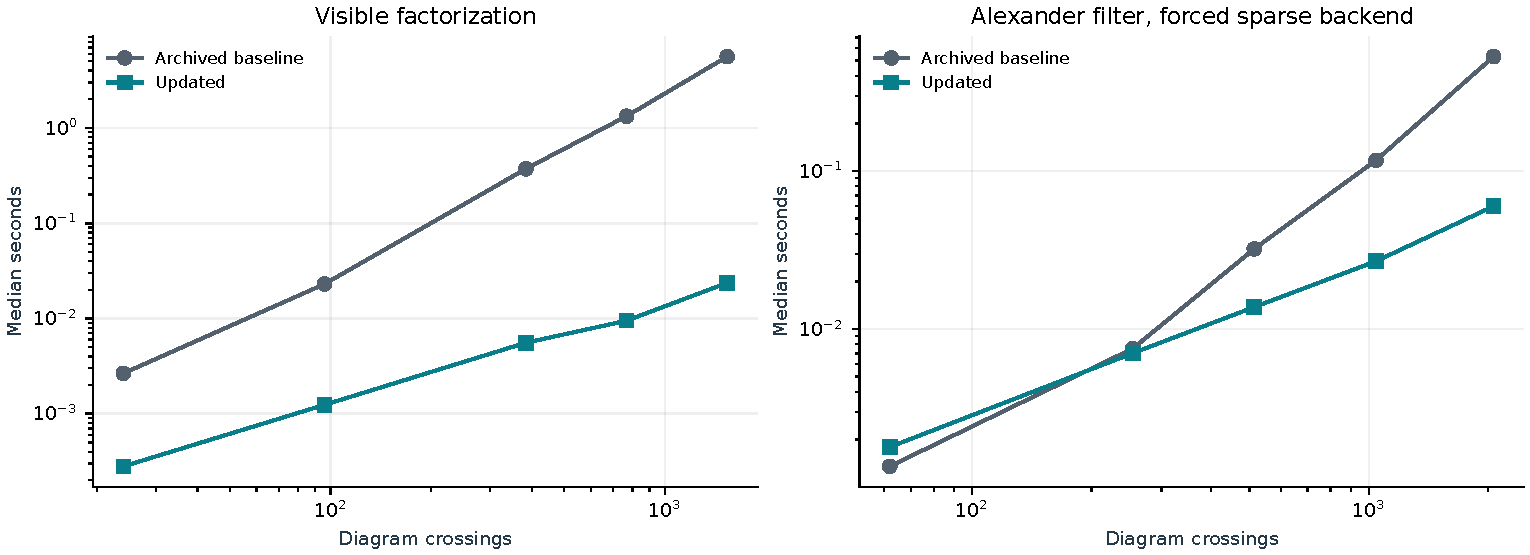
\includegraphics[width=\linewidth]{figures/scaling.pdf}
\caption{Measured scaling on two specified families.  Lines connect sampled
input sizes and are not fitted asymptotic exponents.  The factorization
comparison also has a structural proof; the sparse-family comparison has
a bound in terms of elimination work and measured pivot counters.}
\label{fig:scaling}
\end{figure}

\subsection{Pointed scanning: savings and regressions}

\begin{table}[htbp]
\centering\small
\begin{tabular}{lrrrl}
\toprule
Diagram & $n$ & Baseline ms & Pointed ms & Ratio [95\% bootstrap interval] \\
\midrule
Conway & 11 & 7.671 & 7.762 & 1.046 [0.939, 1.125] \\
Kinoshita--Terasaka & 11 & 6.905 & 7.090 & 1.004 [0.966, 1.069] \\
Hard unknot (8) & 8 & 1.168 & 1.268 & 1.191 [1.015, 1.275] \\
Unknot braid (40) & 40 & 1.683 & 1.948 & 1.114 [1.045, 1.231] \\
Stress closure (36) & 36 & 506.808 & 381.397 & 0.723 [0.673, 0.780] \\
$T(3,11)$ & 22 & 8.225 & 9.300 & 1.119 [1.072, 1.158] \\
Survivor 0 & 16 & 9.382 & 8.597 & 0.921 [0.896, 0.969] \\
Survivor 1 & 15 & 10.704 & 11.902 & 1.054 [1.021, 1.126] \\
Survivor 2 & 15 & 5.453 & 5.728 & 1.094 [1.007, 1.231] \\
\bottomrule
\end{tabular}

\caption{Direct reduced versus ordinary full-rank scanning, with the same
precomputed order.  These timings exclude the recognizer's preceding
filters and do not time early termination.}
\label{tab:pointed-times}
\end{table}

\begin{table}[htbp]
\centering\small
\begin{tabular}{lrrrr}
\toprule
Diagram & Compositions A & Compositions B & Peak objects A & Peak objects B \\
\midrule
Conway & 90 & 56 & 246 & 123 \\
Hard unknot (8) & 0 & 0 & 11 & 11 \\
Stress closure (36) & 23710 & 16705 & 17694 & 12341 \\
$T(3,11)$ & 214 & 75 & 126 & 77 \\
\bottomrule
\end{tabular}

\caption{Selected deterministic scanner counters.  A is the ordinary
scanner; B is the pointed scanner.  Peak objects are measured before
cancellation at each crossing.}
\label{tab:pointed-work}
\end{table}

On the 36-crossing stress closure, compositions decrease from 23,710 to
16,705, peak objects from 17,694 to 12,341, and transferred entries from
251,455 to 173,583.  These are exact work-count changes for the specified
order.  They do not amount to halving the whole computation, and the
timing table confirms that the effect depends on the input.

The three survivor cases are simplified unknot diagrams retained by the
repository's hard-unknot experiment after its filters fail to decide.
They are relevant to the residual decision stage, but have only 15 or 16
crossings.  Their results must not be extrapolated to large difficult
unknots.  The stress closure is useful for measuring substantial homological
work; it is not evidence that the complete pipeline needs homology on
every large input.

\begin{figure}[htbp]
\centering
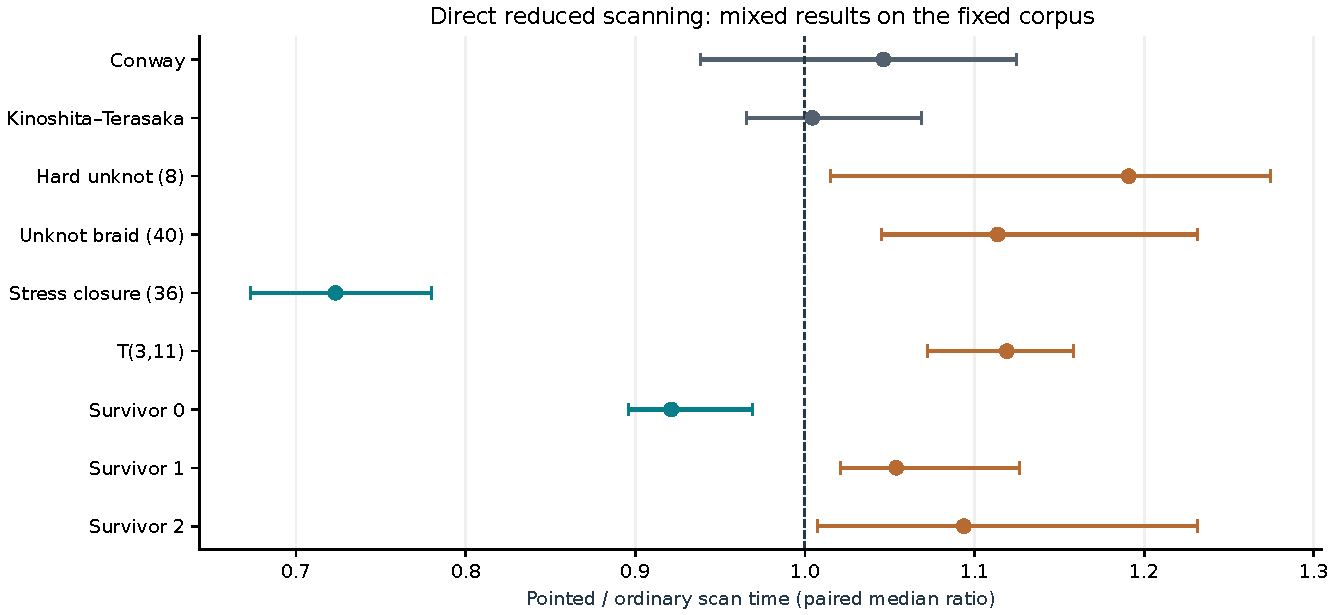
\includegraphics[width=\linewidth]{figures/pointed_ratios.pdf}
\caption{Pointed scan ratios with nominal 95\% bootstrap intervals.
The vertical reference is equal time.  Mixed results support retaining
an explicit \code{--pointed} option instead of changing the default scan.}
\label{fig:pointed-ratios}
\end{figure}

The before-closure examples in Section~\ref{sec:pointed} validate a new
decision mechanism.  They are not added to a headline speedup figure,
because visible factorization already handles those connected sums.  An
honest next experiment should seek prime-looking filter survivors on which
the certificate arises substantially before the last crossing.

\subsection{What the experiment does not settle}

The corpus contains deterministic constructed families and small finite
enumerations.  It is neither a uniform sample of knot types nor a validated
distribution of hard unknot instances.  Relabeled diagrams improve
representation coverage without adding knot types.  Exhaustive braid-word
enumeration similarly contains repeated knots.  Large filter-decided examples
mainly test preprocessing and rejection; a general complexity claim must
also handle large unknots and nontrivial knots that survive all filters.

The remaining quantitative uncertainty is explicit: there is no universal
bound on retained multiplicity, no guarantee of a useful early isolated
summand, no implemented noose certificate for the current order, and no
constructive hierarchy backend satisfying Section~\ref{sec:hierarchy}.
The experiments measure completed changes while leaving these obligations
open.

\section{Further research questions and proposed milestones}
\label{sec:research}

The next stage should pursue two complementary goals: improve the exact
implemented recognizer on difficult inputs, and prove structural statements
strong enough to control its worst case.  The following questions specify
what would count as progress.  They include possible negative results; a
counterexample to an attractive compression hypothesis is useful when it
prevents an unjustified global claim.

\subsection{Q1. Which frontier topology controls matching support?}

The immediate question is whether a useful intermediate bound lies between
the single-disk Catalan estimate and the unrestricted double factorial.
Suppose the processed region has $b$ relevant boundary components.  Can its
realizable matching support be bounded, under a precise encoding of endpoint
orders and boundary incidences, by an expression such as
$2^{O(w)}w^{O(b)}$?  If so, which additional winding or connectivity data
must be retained?  If not, can an explicit planar knot family demonstrate
the obstruction?

The first milestone is a certified boundary representation derived from
the PD rotation system.  The checker should report actual boundary cycles,
the frontier incidences on each cycle, and the processed side.  A second
milestone is a theorem about exactly that representation, tested against
the six-state counterexample and the default Conway-sum fixture.  Counting
abstract noncrossing partitions under a boundary order not supplied by the
input would not meet this milestone.

\subsection{Q2. Can certified noose decompositions replace greedy scans?}

A greedy linear order is easy to run and often effective, but it lacks the
geometric certificate required for the sharper count.  A decomposition based
on embedded separators or nooses could carry that certificate with each
interface.  The design question is how to compose tangle complexes along a
branching decomposition while controlling both width and homological
multiplicity.

The first prototype should expose a checked decomposition format before
optimizing the algebra.  Compare its certified boundary widths, support
sizes, peak multiplicities, and wall-clock cost with the existing greedy
order on identical diagrams.  A low-width decomposition can still lose
through expensive joining operations; the accounting must include those
joins.  A route to \eqref{eq:main-target} needs a structural theorem after
allowed reductions, or a complementary method for pieces that retain large
interfaces.

\subsection{Q3. What compresses repeated tangle complexes?}

Visible two-edge cuts admit a scalar connected-sum rule and are now handled
efficiently.  Four-ended cuts are the next natural extension.  Can a useful
class of tangles be represented by small complexes of boundary modules,
with exact composition and a canonical compressed form?  Repeated tangles
could then share a symbolic representation instead of duplicating all
generators.

The central obstacle is extension data.  The total rank, graded rank, or
Jones polynomial of each piece generally does not specify the differential
or the boundary action needed after gluing.  A proposed summary must therefore
come with a congruence theorem: equal summaries give equivalent results under
every permitted complementary gluing.  Test this property on exhaustive
small tangles with several closures before treating it as an algorithmic
interface.  A compact dictionary of repeated byte-identical complexes can
be an initial engineering step, but is not itself such a theorem.

\subsection{Q4. Can decision certificates appear before full reduction?}

The isolated-summand theorem supplies one exact lower bound, and the
vertex-cover lemma supplies another after scalar closure.  Can they be
extended to small blocks of objects whose every allowed completion has
nonzero reduced homology?  A useful block certificate must survive the
remaining differential and gluing functors, rather than merely count
uncancelled generators.

Implement the scalar support-graph cover bound first and measure its overhead
against the final cancellation it avoids.  Then study small open complexes
with certified nonzero closures.  A compelling positive result would be a
class of prime-looking filter survivors where a bounded-size certificate
arises after only a controlled portion of the scan.  A compelling negative
result would show that an entire proposed class of local certificates can
remain absent until the end despite large eventual rank.  Neither outcome
requires pretending that the present connected-sum examples establish new
pipeline superiority.

\subsection{Q5. Can the pointed backend be selected cheaply?}

The last-crossing edge policy has a proved frontier property, but it is not
an optimal basepoint theorem.  Which inexpensive statistics predict when
the quotient's savings exceed its bookkeeping?  Candidate statistics include
the time of first marked-edge appearance, early matching multiplicities,
the distribution of equal-matching pivots, and the number of marked surface
components in compiled plans.

A selection rule should be trained or tuned on one corpus and evaluated on
a separate corpus.  Its entire cost belongs in the end-to-end timing.
Running both expensive scans merely to choose the faster one is not a
low-cost selector, although a deliberately bounded race may be useful under
a stated resource policy.  Further algebra work could seek a fused ordinary
and pointed transfer routine that shares topology compilation without mixing
the incompatible numeric cache bases.

\subsection{Q6. Which Alexander matrices have controlled elimination work?}

The sparse theorem reduces a performance question to the actual pivot
parameter $F$.  Can knot-diagram structure, a braid decomposition, or an
embedded separator order imply a useful bound on $F$ for a specified pivot
policy?  Input sparsity does not suffice.  Nor does good behavior on the
sampled $T(3,q)$ diagrams prove that a degree heuristic always maintains
small neighborhoods.

A first theoretical target is a rigorously specified diagram family for
which the pivot evolution can be described inductively.  A second is a
parameterized fill bound in terms of a checked graph decomposition of the
minor's incidence pattern.  Engineering comparisons should include row-only
sparse elimination, indexed complete pivoting, and dense fallback at the
same field and evaluation points.  Track attempted Schur positions and
transient storage, not only newly created fill.

\subsection{Q7. Can preprocessing expose hidden decomposition?}

Interlacement components characterize visible summands of a fixed diagram.
They do not solve topological prime decomposition.  Can a bounded collection
of Reidemeister or flype-like transformations expose enough decompositions
to bound the largest residual piece on a useful class of inputs?  What
certificate shows that the transformation sequence preserves the knot and
that its search cost is controlled?

One intermediate result would bound the work needed to expose a specified
class of obscured connected sums.  A stronger result would control the
size or width of every remaining factor after a proven reduction strategy.
The algorithm must charge unsuccessful move searches and revalidation,
not just successful crossing reductions.  Memoizing repeated factor PD
codes is useful, but it cannot identify arbitrarily disguised equivalent
summands without further mathematics.

\subsection{Q8. Can a geometric hierarchy meet the state-volume contract?}

Section~\ref{sec:hierarchy} gives a quantitative target:
$\sum_i\log(g_i+1)=O(\log^2 n)$, together with polynomially bounded
epochs, encoded data, and total work per charged visit.  Can an accelerated
hierarchy construction prove that complete contract?  This asks more than
showing termination or a short final certificate.

The first deliverable should be a specification of the state, each
transition, its preconditions, and a verification procedure for its output.
Uniform caps must survive every suffix rebuild.  If a decomposition is
restarted with different caps or a different depth, identify and charge a
new epoch.  Unequal caps and unequal level costs should be retained because
the sharp weighted formula can reveal where work is actually concentrated.
A bound of $O(\log^3 n)$ on the logarithmic state volume would still yield
quasi-polynomial time, but would not be the sharper
$n^{O(\log n)}$ claim.

\subsection{Q9. Can compressed geometry stay compressed through every step?}

Interval orbit counting and binary normal coordinates are useful primitives,
but a chain of routines can lose their advantage at an interface.  Can the
algorithm cut, trace components, transport discs, and rebuild boundary
patterns while retaining compressed multiplicities and explicit bit bounds?
Which routines require an actual list of components, and can that output
be represented by types with multiplicities instead?

Implement a small end-to-end path from a triangulated exterior through one
certified cut and back to a valid handle or triangulation description.
Record input and output bit lengths, represented surface weight, number of
interval identifications, and total primitive calls.  Reject an interface
that silently expands a binary weight into one object per normal disk.
Only after this path is specified should a global hierarchy runtime be
inferred from its building blocks.

\subsection{Q10. What benchmark corpus tests the unresolved decision stage?}

The next corpus should contain growing families of known unknots and
nontrivial knots that survive the complete inexpensive front end.  It should
include alternative diagrams of the same knot, certified move traces for
scrambled unknots, high-width examples, and cases with no visible factors.
Crossing number, effective width, boundary topology, matching support,
object multiplicity, and the deciding stage should all be recorded.

Generated instances need provenance.  A known unknot produced by a verified
move sequence supplies a trusted label; a knot that a cheap invariant
rejects measures a different part of the pipeline.  Separate instances used
for heuristic tuning from those used for evaluation.  Fixed seeds,
randomized paired timing, A/A controls, and retained failures should remain
standard.  The purpose is to identify the remaining mechanism of growth,
not to maximize an average speedup on easily rejected diagrams.

\subsection{Q11. Which certificates should be formalized first?}

The shortest independently verifiable components offer a practical entry
point for proof-assistant work: the interlacement spanning forest and nesting
verifier, the inherited-PD reconstruction, finite-field Schur elimination
with permutation signs, and the mixed-radix ranking and suffix budget.
These have explicit finite data and compact mathematical invariants.

For homology, a later stage can formalize the marked-dot ideal and the
surface-evaluation rules, then Gaussian cancellation and its interaction
with gluing.  The distinction between an isolated-object replay record and
a compact chain-equivalence certificate should remain explicit.  A small
formal checker is more useful than a formal statement whose hardest
topological or complexity premise is hidden in an unimplemented oracle.

\subsection{Proposed order of work}

The first implementation milestone is to integrate the audited factorizer
and sparse filter, preserve the pointed option, and establish the expanded
corpus and counter instrumentation.  The first structural milestone is a
certified interface representation with a proved matching-support bound.
The next algebraic milestone is an exact compositional compression or an
earlier decision certificate that handles a substantial residual class.
In parallel, the hierarchy route needs a small compressed geometric backend
whose complete costs can be charged to the explicit ranking model.

A claim of general quasi-polynomial recognition becomes justified only when
every input is covered by one sound, complete algorithm with a proved
worst-case budget.  Combining fast filters with a conditional scanner and
an unspecified hierarchy subroutine does not yet supply that coverage.
The present package gives concrete improvements and testable mathematical
obligations for the next iteration.

\section{Artifact organization and repository integration}
\label{sec:artifacts}

The ZIP is a self-contained research handoff.  Its top-level README specifies
the pinned revision, supported commands, integration paths, and the distinction
between original measurements and final audit reruns.  All performance tables
and plots in this article are generated from retained JSON rather than
transcribed by hand.  The included source files and SHA-256 manifest make
the handoff reviewable independently of the conversation that produced it.

\begin{table}[htbp]
\centering\small
\begin{tabular}{P{45mm}P{97mm}}
\toprule
Path & Purpose \\
\midrule
\path{article/} & Modular \LaTeX{} source, bibliography, compiled PDF,
generated tables, and vector/PNG figures. \\
\path{fast/} & Complete proposed Python package, with existing examples
and tests plus the new implementations and regression tests. \\
\path{baseline/fast/} & Byte-verified original files needed to execute
the archived comparison package. \\
\path{tools/} & Independent finite auditors, paired timing scripts,
table/figure regeneration, article build, and package verification. \\
\path{data/} & Raw measurements, deterministic validation records,
source provenance, final test output, and concise benchmark summaries. \\
\path{integration/} & A patch against the pinned repository paths and
notes on applying or adapting it. \\
\path{SHA256SUMS} & Hashes of packaged deliverable files; the manifest
does not hash itself. \\
\bottomrule
\end{tabular}
\caption{Research package layout.}
\end{table}

\subsection{Public behavior and compatibility}

The default recognizer now uses the checked interlacement factorizer.
The old \code{visible\_factors} function remains unchanged, and
\code{factor\_backend="legacy"} or the CLI's \code{--legacy-factor}
selects it for comparison.  New factorization evidence is a component
certificate under \code{connected\_sum\_factorization}; callers that parse
the old geometric cut trace should use the legacy backend or adopt the
new documented evidence schema.  This schema change is deliberate and
must be considered during integration.

The Alexander obstruction retains its previous witness dictionary.  Its
new backend and statistics arguments are optional.  Existing callers need
not supply them.  Dense elimination remains the reference implementation.
The runtime-budget callback now reaches sparse pivots and the factorization
stage; limits are cooperative and can still be exceeded inside an operation
without an intermediate callback, such as validation or exact polynomial work.

\code{--pointed} is an explicit recognizer option.  It currently requires
min-fill pivots, bit algebra, no deferred tail, and one scan order rather
than a race.  Incompatible CLI options receive an input error; the Python
API raises \code{ValueError}.  The direct
\code{reduced\_khovanov\_rank} result stores a \emph{reduced} rank in both
\code{rank} and \code{reduced\_rank}, and reduced values in
\code{by\_degree}.  This differs intentionally from the original
\code{khovanov\_rank} interface, whose \code{rank} is unreduced.

The separate \code{reduced\_khovanov\_decision} can return
\code{reduced\_rank=None} with a certified lower bound and replay data.
Clients must not interpret that lower bound as an exact rank.  Existing
full-rank APIs, including the legacy factored-rank helper, retain their
semantics.  The package does not silently enable pointed scanning for them.

\subsection{Reproducing the checks}

From the unpacked top-level directory, the following commands run the main
verification programs.  Explicit output names avoid overwriting the retained
research records.

\begin{lstlisting}
PYTHONPATH=fast python3 -m unittest discover -s fast/tests -v
python3 tools/verify_factorization.py \
  --output data/reproduced_factorization.json
python3 tools/verify_reduced_scan.py \
  --output data/reproduced_reduced.json
python3 tools/verify_frontier_counterexamples.py \
  --output data/reproduced_frontiers.json
python3 tools/hierarchy_budget.py --self-test \
  --output data/reproduced_hierarchy.json
python3 tools/verify_package.py
\end{lstlisting}

The recognition code and finite auditors use only the Python standard
library.  Matplotlib is needed only to regenerate figures; pre-generated
figures are included.  Building the article requires a conventional
\LaTeX{} installation with the listed packages and BibTeX, conveniently
driven by \code{latexmk}.

\begin{lstlisting}
python3 tools/render_results.py
sh tools/build_article.sh
PYTHONPATH=fast python3 -m fastunknot recognize \
  fast/examples/conway.json
PYTHONPATH=fast python3 -m fastunknot recognize \
  fast/examples/conway.json --no-alexander --no-jones --pointed
\end{lstlisting}

The benchmark README gives the timing commands, source selection, and
expected runtime considerations.  Timing scripts intentionally perform
real repeated computations and are separate from the quick regression
suite.  Reproducing exact operation counts is a stronger expectation than
reproducing identical elapsed times in a shared environment.

\subsection{Integration boundaries}

Apply the supplied patch only after checking the target revision.  If the
repository has advanced, review the differences around the touched Python
modules rather than treating the archived patch as authoritative over later
work.  The updated \path{fast/} directory is also supplied as an ordinary
source tree, so the intended changes can be inspected without applying a
patch.

Place the article and its accompanying tools/data under a new dated research
directory in \path{Topology/UnknotRecognition}, or use the repository's
preferred publication layout.  The existing synthesis remains a historical
record; the new article supplies the frontier-count correction and updated
literature status.  The bundle includes the repository's MIT-0 license.
No remote commit, pull request, or publication is required to inspect or
reproduce this handoff.


\clearpage
\bibliographystyle{plainnat}
\begingroup\raggedright
\bibliography{references}
\endgroup
\end{document}
